\documentclass{article}
\usepackage[a4paper, left=1.85cm, right=1.85cm,top=1.85cm, bottom=1.85cm]{geometry}
\usepackage[utf8]{inputenc}
\usepackage{float}
\usepackage{times}

\usepackage{afterpage}
\date{\vspace{-5ex}}
\usepackage[sorting=none]{biblatex}
\usepackage[utf8]{inputenc}
\usepackage[english]{babel}
\usepackage{graphicx}
\usepackage{float}
\usepackage[style=plain]{floatrow}
\addbibresource{name.bib}
\usepackage{amsmath}
\usepackage{gensymb}
\usepackage{dirtytalk}
\usepackage{amssymb}
\usepackage{graphicx}
\usepackage{caption}
\usepackage{subcaption}
\usepackage{chngcntr}

\usepackage{fancyhdr}

\pagestyle{fancy}                           % Insert header
\renewcommand{\headrulewidth}{0pt}
\lhead{Team Project 5}                          % Your name
\rhead{James Cook University Hospital - NHS South Tees}

\begin{document}

%\end{document}
\vspace{-10mm}

\counterwithin{figure}{section}

\counterwithin{table}{section}

\begin{titlepage}
   \begin{center}
       \vspace*{1cm}

       \textbf{\large A Thermodynamic Analysis of Neonatal Incubators}

       \vspace{0.5cm}
        Level 3 Team Project, James Cook University Hospital, \\ NHS South Tees, Dr Prakash Loganathan
            
       \vspace{1.5cm}

       \textbf{Lochlan J.L. Shillington, Freddie H. Britt, Jonny R. Gutteridge, Gina Hooton, \\ Ben Turner-Tatman, \& Josh K. Read}

       \vspace{5cm}

       
\includegraphics[width=0.5\textwidth]{Durham.jpeg}
            
       Department of Physics\\
       Durham University\\
       United Kingdom\\
       Date: \today{}
        
        
   \end{center}
   
   
\end{titlepage}


\tableofcontents

\newpage

\section{Executive Summary}
Our project brief set our team a series of five questions related to the use of hospital incubators, primarily focused on the GI Giraffe incubator: 

\vspace{3mm}

\noindent 1. How BABY MODE/SERVO MODE adjusts the temperature? 

\vspace{2mm}

\noindent 2. How NHS doctors or nurses should be adjusting the temperature when using AIR MODE?

\vspace{2mm}

\noindent 3. How much heat loss is happening when one or more side (porthole) doors are opened? What is the impact with duration of door opening? 

\vspace{2mm}

\noindent 4. What is the efficacy of “AIR BOOST” when it is activated?

\vspace{2mm}

\noindent 5. What is the impact of humidity on the temperature control? 

 \vspace{3mm}

In order to evaluate these questions, a series of seven thermocouples and two humidity meters were placed throughout both the GI Giraffe incubator and an associated acrylic model. The ‘air mode’, ’air boost’ and ‘servo mode' incubator settings were all tested under varying temperature and humidity conditions to determine some conclusions about them. 

 \vspace{3mm}

Experiments were conducted to measure the ability of the incubators in maintaining the temperature and humidity in ‘air mode’, ‘air boost’ and ‘servo mode', each for 20-minute intervals. This provided a series of results summarised below: 

\vspace{3mm} 

Servo mode is mostly used in the first two weeks of a neonatal baby's life, when they are not developed enough to maintain their own body temperature. The servo mode experiments proved that the incubator responds proportionately to the temperature difference between the baby’s skin and the set temperature of the incubator. As this temperature difference increases, the speed of the temperature response and the magnitude of the response increase too. The incubator was effective at both increasing and decreasing the inside temperature. However, it was found to be more effective at increasing the temperature than decreasing it. One of the key findings was that temperatures in different locations of the incubator could be up to 5$^{\circ}$C different, causing the temperature to become too high in certain locations. 

\vspace{3mm}

Air mode is used in the later stages of a neonatal baby’s life when they are more thermally stable. During air mode experiments, the most significant source of heat loss was through the end of the incubator. This is likely due the heat loss through the multiple small openings at the end of the incubator. Furthermore, when the portholes are open, the rate of humidity decrease was significant within the first minute of opening the portholes.  

 \vspace{3mm}

For air mode, the rate of temperature decrease for the model baby when the porthole doors were open was negligible at the rate of (-1.03 $\pm$ 0.06) $\times$10$^{-3}^{\circ}$Cs$^{-1}$ at a high humidity setting. However, despite setting the target temperature of the incubator to 37.0$^{\circ}$C, the temperature of the baby remained at a critical temperature of approximately 35$^{\circ}$C which poses a significant health risk of hypothermia. Therefore, air mode was unable to increase the temperature of the baby to the target temperature and a higher target temperature is recommended when the portholes need to be opened. 

 \vspace{3mm}

At a lower humidity setting, the effect of heat loss during air mode was slightly reduced, reaching a higher minimum temperature than when the same experiment was conducted in a higher humidity setting. The air from the heater was able to escape less through the porthole door openings and contribute more towards the convection currents in the incubator. However, this had negligible effect on the temperature of the baby as the temperature continued to decrease at a rate of (-1.53 $\pm$ 0.01) $\times$10$^{-4}^{\circ}$Cs$^{-1}$. Although this rate is negligible, the temperature of the model of the baby was unable to reach the target temperature. 

 \vspace{3mm}

Air boost mode is designed to retain heat while portholes are open. Air boost was found to decrease the humidity inside the incubator more than in air mode. The relative humidity reached a low of 47\% in air mode during a 20-minute data set with 4 portholes open, whereas an equivalent set of data for air boost caused the humidity to drop to 43\%. However, there is evidence to suggest that air boost does maintain temperature inside the incubator more efficiently than air mode - the Heat Sensor thermocouple experienced a low of 36.5$^{\circ}$C in a 20-minute period with 4 portholes open in air mode, whereas air boost saw a low of 37.5$^{\circ}$C, suggesting better heat retention. 

 \vspace{3mm}

Several improvements to the incubators were devised. These improvements aimed to resolve two problems: the servo mode temperature probe falling off the baby, and the rapid heat and humidity loss when portholes are opened for medical interaction. Intending to decrease heat and humidity loss, a design involving rubber sleeves attaching to the portholes was trialled, with experimental evidence indicating a significant increase in humidity retention. For the unmodified incubator, the smallest temperature decreases were greater than 10.7$^{\circ}$C, however in the 'sleeve-modified trials’, the largest drop was only 10.56 $\pm$ 0.06$^{\circ}$C. Hence the greatest drop in temperature with the sleeves was equal to the smallest drop without them, suggesting significant improvement. 

\section{Introduction}

Premature babies will naturally have poor thermal regulation systems. This is because they have not developed as much as regular new-born babies, and therefore have a lack of body fat, a limited metabolic rate, and a higher surface area to volume ratio. As a result, heat transfer out of a premature baby is relatively high, but the baby is unable to produce the energy it requires to maintain its own body temperature. This means that premature babies are especially prone to hypothermia, which is a serious risk to their health in the early days of their life. 

\vspace{3mm}

Hospitals use incubators to help premature babies maintain their body temperature. At James Cook Hospital, the incubator systems have two different “modes” that are used to control temperature inside them. The first is called 'Air mode', whereby the nurse can set a specific temperature (to the nearest 0.1°C) and the incubator system maintains that temperature inside by measuring the temperature with a built in sensor and adjusting the temperature of the air going into the incubator accordingly to ensure the incubator stays at the desired temperature. As part of this mode, there is an additional setting called ‘Air boost’ which is designed to maintain temperature when the doors are open. The second mode is called ‘Servo mode’. In this mode, a temperature probe is attached to the skin of the baby, and rather than inputting a desired temperature of the air, the nurse inputs a desired temperature of the baby. The computer system then changes the temperature of the incubator heater depending on the measured temperature of the baby in order to keep the baby temperature as close to the correct temperature (37°C) as possible. 

\vspace{3mm}

Although the incubators are generally very successful at keeping prenatal babies alive, the hospital have suggested ways in which the system is sometimes less effective. Firstly, the probe that is attached to the skin of the baby during servo mode must be stuck with a gel-based sticker. The gel base ensures that the sticker does not damage the skin of the baby, which is thin and fragile at this age, but due to the moistness of the baby’s skin, the sticker can sometimes become unattached. As a result, the temperature probe can measure a different temperature to the actual baby temperature and causes the servo mode system to alter the temperature inappropriately high or low. Additionally, it is suggested that a small change in temperature of the baby can cause servo mode to change the air temperature very drastically. Currently, the doctors do not know what these temperature changes look like. Another issue is that the incubators need to have their portholes opened for certain procedures. For example, babies usually need to have a catheter inserted into their umbilical cord. According to the staff at the hospital, this can take between 20-60 minutes and requires all four incubator doors to be opened for the duration of the procedure. This could be causing significant heat losses in the incubator that the doctors are unaware of.

\vspace{3mm}

The primary aim of this project, as requested by Dr Prakash Loganathan at James Cook Hospital, is to try and improve the understanding of how the different modes of the incubator work from a thermodynamics perspective. Specifically, Dr Loganathan asked the team to examine exactly how the temperature changes inside the incubator during servo mode and how the mode adjusts to temperature changes of the “baby” it is attached to. He also wanted the team to investigate the heat losses that occur when opening the portholes of the incubator, find out the best way of adjusting air mode, work out the efficacy of the air boost function and evaluate the impact of humidity on the temperature control. An additional aim of the project has been to find any suggested improvements that could be made to the incubator, and although this has not been the focus of the project, it is still something that has been considered.

\section{Thermodynamic Model}\label{Thermodynamic}

By using a series of physical assumptions, an attempt will be made to create a model of the baby-incubator system to justify our systematic set-up. 

\vspace{3mm}

A typical premature neo-natal child has a specific heat capacity of 3515 J kg$^{-1}$ $^{\circ}$C$^{-1}$ \cite{BTT1} meaning a child will on average store 3515J of energy per degree of its temperature per kilogram of mass.  This value allows us to work out how the temperature of the neonate fluctuates as it loses heat energy to a cold surrounding. The average heat loss per second of a neonate was determined to be between 20 and 40 W m$^{-1}$ kg$^{-1}$. It was decided to take the two extreme values (with case 1 being 20W and case 2 being 40W) given by the Bolin and Holmér \cite{BTT5}. The decision to use a 1kg mass was based on research  by the American Association of Pediatrics \cite{BTT4} suggesting that the average 28-week-old neonate weighs approximately 2.3lb (1kg). This mass was believed be the most useful compromise, as the results would be focused on the prenatal infants with the highest risk of temperature loss whilst still being applicable to those of more moderate weights. Similarly, based on the work of Ostrowski and Rojczkye \cite{BTT2} the effective surface area (the area in contact with the surrounding air, not including the section of the baby in permanent contact with the incubator bed) of the baby was taken to be 0.107m$^{2}$.  This provides an energy loss for the simulated baby in case 1 as 4.28W and case 2 as 2.14W.    

\vspace{3mm}

It has further been estimated that heat energy gain of all metabolic process in neonatal children is 2.25$\pm$0.06 W kg-1 \cite{BTT9}, which for a 1kg child is simply 2.25$\pm$0.06 W. By subtracting these values, the net heat leaving the child, Z, for case 1 is –0.11$\pm$0.06 W and for case two it is 2.03$\pm$006 W. Due to the range in heat loss values, it is possible for babies to act either as a heat source (emitting more heat than they take in for the environment) if Z is positive, or a sink (taking in in more energy from the surroundings than they emit) if Z is negative. However, in high temperature environments within an incubator, due to the overall lack of metabolic processes occurring in the youngest premature infants, it is more likely for a baby to behave as a heat sink than a heat source \cite{BTT7}. Therefore, it is feasible to approximate a baby at temperatures approaching and above that of an incubator as a material of a set initial temperature, that does not produce any heat besides its initial temperature. To show this the specific heat capacity equation may be used , 


\begin{equation}\label{a}
    c=\frac{\Delta Q}{m \Delta T},
\end{equation}


where c is the specific heat capacity of our material, m is the mass of the material, $\Delta$Q is the change in heat and $\Delta$T is the change in temperature.  The density of air is approximately 1.20 kgm$^{-3}$  \cite{BTT7} and its specific heat capacity is 7.18 J kg$^{-1}$ °C$^{-1 }$.

 \vspace{3mm}

In the case of a Giraffe incubator, and our respective model of it, the volume of air in the incubator was determined to be 0.173m$^{3}$, and thus the mass was found to be 22.3 kg. However, it will have a higher mass in an actual incubator due to a higher humidity level. To initially heat the air in the incubator from room temperature 21.0°C to 37.0°C., the heat energy required was determined to be 2470 J. This value far exceeds the energy emitted by the neonate per second at 3.21 Js$^{1}$  and is far less than the running power of an Incubator at 300W(the majority of which is used on heating) \cite{BTT8} indicating the heat produced by a baby internally is negligible within an incubator. Further, the average temperature of the PVC of an incubator box with internal temperature 37.0°C was determined using a series of images produced by the thermal imaging camera. 

\begin{figure}[H]
\centering
\begin{minipage}{.48\linewidth}
    \captionsetup{justification=centering,margin=0.1cm}
    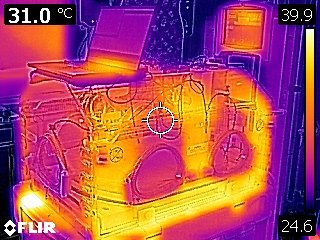
\includegraphics[width=\textwidth]{Sample Thermal Imagining Camera.jpg}
    \caption{example image of the GI Giraffe Incubator at James Cook Hospital taken using the FLIR C2 thermal camera .}
\end{minipage}
\hfill
\end{figure}
By analysis of these images, a surface temperature of 34 $\pm$ 1°C was approximated suggesting a high degree of heat loss to the surroundings given the high level of heat on the surface of the PVC. 
\vspace{3mm}
 
 \begin{figure}[H]
\centering
\begin{minipage}{.48\linewidth}
    \captionsetup{justification=centering,margin=0cm}
    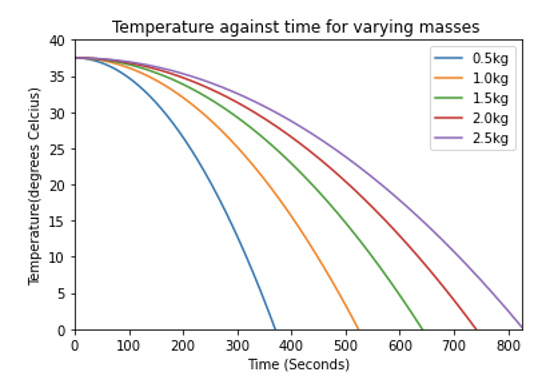
\includegraphics[width=\textwidth]{1.png}
    \caption{ Plot of Temperature against time for 5 different masses indicative of a range of small neonatal babies. }
    \label{Mass diff}
\end{minipage}
\hfill
\begin{minipage}{.48\linewidth}
    \captionsetup{justification=centering,margin=0.6cm}
    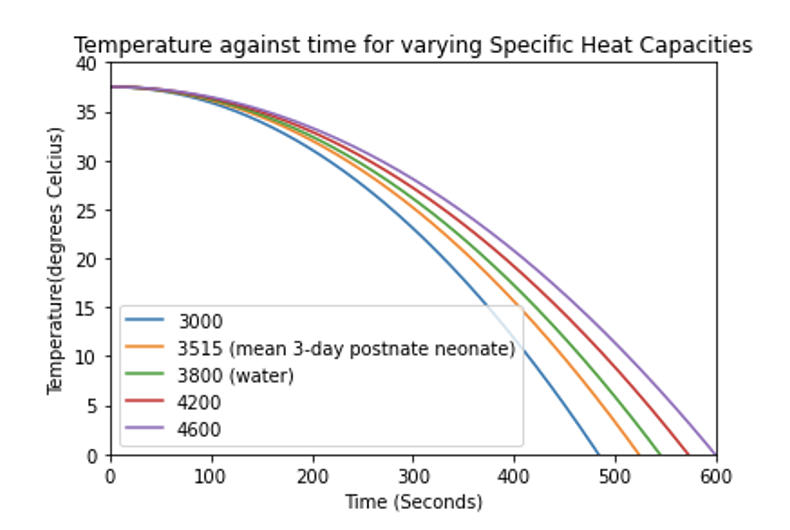
\includegraphics[width=\textwidth]{2.png}
    \caption{Plot of Temperature against time for 5 different specific heat capacities. }
    \label{Heat Capacities}
    \end{minipage}
\end{figure}

To demonstrate the impact of weight and specific heat capacities on babies' ability to maintain temperature, range of masses (0.5, 1.0, 1.5, 2.0, 2.5kg) was plotted, keeping specific heat constant at 3151 J kg-1 °C$^{-1}$ . Various specific heat capacities were also plotted (3000, 3515, 3800, 4200, 4600 J kg$^{-1}$ °C$^{-1}$) for a mass of 1kg for a new-born in a cold reservoir (an environment that has an ability to indefinitely take heat from the baby without reaching a thermal equilibrium with the baby, such as a large room significantly below freezing). This is done by using Eq. \ref{a} with the initial temperature set at 37 $^{\circ}$C. 

\vspace{3mm}

Fig.\ref{Mass diff} depicts a large variation of times required for the masses to reach 0 $^{\circ}$C, with the 0.5 kg mass taking 383s and the 2.5kg mass taking 832, twice that of the smallest. Fig. \ref{Heat Capacities} shows the graph depicts a much smaller variation of times required for the masses to 0$^{\circ}$C, with the all heat capacities grouped within 117 seconds. 

\vspace{3mm}

After analysing the results of Fig. \ref{Mass diff} and Fig. \ref{Heat Capacities}, a decision was made to describe the model baby using water, as in the range of data 25-35$^{\circ}$C the two specific heat value behaved so similarly as to effectively approximate each other. This is to be expected as the water content of neonatal children is in the range 75-80\% \cite{BTT3}. The decision was in response to a difficulty in using a mixture of fluids that could effectively emulate the exact postnatal value. One solution was suggested a graphit-33 spray \cite{BTT2} on the plastic resealable bag containing the water to reduce the thermal conductivity, however due to the inability to  prevent the graphit-33 from de-adhering and contaminating the hospital incubators this was not adopted. The mass of the resealable bag was measured as $2 \pm 0.5$g and thus taken as negligible for the total specific heat capacity as the thermal mass of the object will be insignificant.  

\vspace{3mm}

The decision to use a 1kg mass was based on research by the American Academy of Pediatrics \cite{BTT4} suggesting that the average 28-week-old (gestational age) weighs 2.3lb (1kg). This was found be the best balance, as our results would be focused on the premature babies with the highest risk of temperature loss whilst still being reasonably applicable to those of more moderate weights (1.5-2kg). The simulated data also implies that as neonatal babies develop, the thickness of their skin and associated increase in specific heat capacity is less significant than the increase of mass for heat retention. However, notably this model cannot account for the variance of sweat production and associated trans-epidermal water loss (TEWL).  

\vspace{3mm}
TEWL is the loss of water across the skin (epidermis) passively through osmotic pressure and is commonly measured in gm$^{-2}$h$^{-1}$ \cite{BTT1}. The primary factors in determining the rate of TEWL are the humidity of the environment, thickness of skin and surface area to volume ratio. As a baby develops, its surface area to volume ratio decreases, and the thickness of skin increases. These factors all contribute to a decrease in TEWL which is measured per m$^{2}$ of surface area as age increases.  
\begin{figure}[H]
    \centering
    \captionsetup{justification=centering,margin=1cm}
    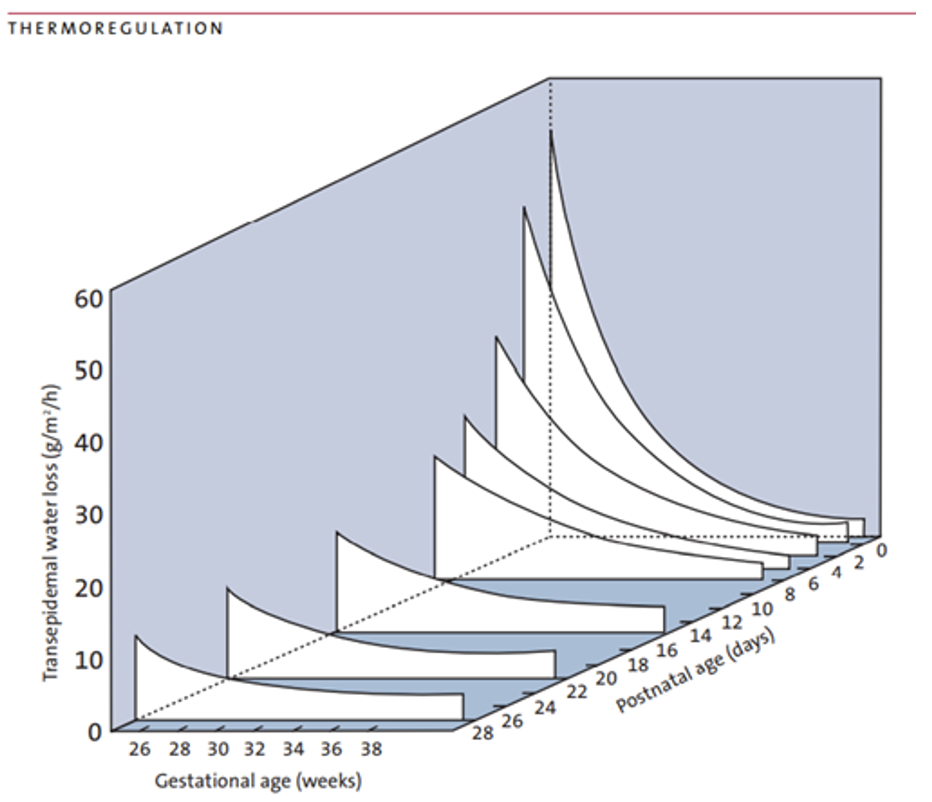
\includegraphics[width=0.5\textwidth]{3.png}
    \caption{Credit: \cite{BTT1} 
    The relationship between the age of a child, both gestational age (time since mother’s last menstrual period) , postnatal age(time since birth) and trans-epidermal water loss (TEWL).  This shows that for both early gestational and postnatal ages there is an incredibly high TEWL indicative of poor fluid management across the skin membrane.  }
    \label{TEWL}
\end{figure}


As Fig. \ref{TEWL} demonstrates, there is a wide range in TEWL across gestational and postnatal ages, therefore, an added factor accounting for age and water loss would improve estimations of temperature loss in babies. However, models of specific heat capacity cited do not specifically refer to age (but rather mass), so to combine these models more work should be done on the correlation between age, specific heat capacity, mass, and TEWL. It is likely there is an even greater variance between low mass, low age babies and their older and heavier counterparts than predicted in the model used at Durham University. 

\vspace{3mm}

As noted above, due to osmotic pressure, the rate of TEWL will be highly dependent on humidity, so in an environment with uncontrolled humidity these values are liable to fluctuate. Similarly high humidity would be the best way to reduce TEWL. This suggests that humidity is likely to not only be a key factor in preventing dry skin and stabilising the total incubator temperature but also causing neonatal babies to maintain a more stable temperature internally, irrespective of external temperature. 

\vspace{3mm}

It’s worthwhile thinking about the incubator and baby as a thermodynamic system in order to predict the way in which it will cool down. The surroundings of the incubator (the hospital ward or any other room the incubator might be in) will be at a lower temperature than the incubator itself, as an ambient temperature of less than 37 °C (approximately) necessitates the use of an incubator. The volume of the surroundings will be very large in comparison to the volume of the incubator itself (the incubator that this project investigates has a volume of 0.173 m$^{3}$, as calculated in Sec. \ref{Thermodynamic}, and as such is very small in comparison to the larger hospital ward that could be of the order 10$^{2}$ m$^{3}$) and can be therefore treated as an infinite thermodynamic cold sink. Furthermore, the ward will have its own independent heat regulation system, meaning it is even less likely to waver in temperature in comparison to the incubator. Any heat dissipated by the incubator can be assumed to not add heat to the surroundings.  

 \vspace{3mm}

Heat can be lost from a system in three different ways, all of which were expected to play a part in the cooling of the incubator: 

\begin{itemize}

\item Conduction – the transfer of energy via collisions of molecules \cite{JG1}. Energy will be transferred from the higher temperature (higher energy) substance to the lower temperature one. In our system (baby, incubator, surroundings), the molecules of air within the incubator are the most energetic as they are the highest temperature. They will transfer energy to the baby and the incubator walls through these energetic collisions. The walls of the incubator, once at a temperature higher than that of the surroundings, will lose heat via conduction with the surrounding air. 
 \vspace{1.5mm}
 
\item Convection – the loss of heat from a fluid through movement and subsequent cooling \cite{JG2}. In our system, the hottest air inside the incubator will rise due to it being less dense, travelling further from the heaters and cooling at the top of the incubator. The heat from the hot air is transferred to the incubator walls, which then transfers to the surroundings via conduction. 
 \vspace{1.5mm}
 
\item Radiation – heat emitted in the form of electromagnetic radiation \cite{JG3}, most commonly in the infrared region for a warm object. In our system, any warm object will emit infrared radiation which will travel into the surroundings. Infrared / thermal cameras are responsive to infrared light, showing the user the sources of infrared radiation in the image, and hence the hottest objects. Thermal images have been captured throughout out data taking (see Sec. \ref{Thermodynamic}). 

 \end{itemize}

Care was taken throughout the data-taking process to ensure humidity was set to the correct value. Figs. 6.1 and 6.3 show the impact of low humidity on cooling of the incubator - see Sec. \ref{ModeBoostComparison} for relevant analysis. As such, humidity was controlled for comparable data sets.  

 \vspace{3mm}

Humidity, or relative humidity, is a measure of the quantity of water vapour in a given volume of air. This is often referred to as a percentage, with 0\% being no water vapour and 100\% being the maximum amount that the air can hold at that specific temperature, pressure, and volume. 

 \vspace{3mm}

Temperature impacts the amount of water vapour that a certain volume of air can hold. The saturated vapour density is the maximum mass of water vapour that 1 cubic metre of air can hold at a given temperature, often referred to in grams per metre cubed (gm$^{-3}$). The higher the temperature of the air, the higher the saturated vapour density.

 \vspace{3mm}

As stated earlier in this section, the incubator that this project focusses on has a volume of 0.173m$^{3}$. At 37$^{\circ}$C, the saturated vapour density is 44gm$^{-3}$ \cite{JG6}. Therefore, for 25\% humidity (25\% of the maximum total humidity per metre cubed), the air inside the incubator will contain 1.90g (3 s.f.) of water. Additionally, a humidity of 75\% will contain 5.71g of water, approximately 3 times more.  

 \vspace{3mm}

The rate at which the incubator will cool will be lower at a higher humidity. The internal energy of the system will be significantly greater at 75\% humidity compared to the 25\% case as there is 3 times the water (at 37$^{\circ}$C) that contains additional internal energy. Hence humidity has a key role in the retention of heat in the incubator and as such, should be measured and considered during the experiments. 

\section{Methodology} \label{MethodSection}

 In general, the experiments have been designed to measure the temperature of the incubator at several different positions (simultaneously) for periods of 20 minutes. The majority of experiments were conducted at James Cook hospital, but some have also been conducted on a model incubator in the Durham University physics laboratories.

\vspace{3mm}

 The incubator that the team worked with at James Cook hospital is the Giraffe Carestation CS1. The incubator has five portholes and has both air mode and servo mode technology (Fig. \ref{Fig 2.1:}).

\vspace{3mm}

 In order to conduct experiments in the laboratory at Durham, a model of the incubator has been made. To do this, the specifications shown in Fig. 11.2 (found in Sec. 11.3) were sent to Bay Plastics Ltd, a local plastic company, and they were able to build the model shown in Fig. \ref{fig:durhamModelPic}. The model was made from 6mm thick acrylic. The porthole cut-outs had been sent along with the model, and electrical tape was used to stick these into place when necessary for the experiments. The team was unable to get servo mode or air mode systems into the laboratory due to a lack of a built-in heating element, as explained in the Sec. 5 (Limitations). However, a 2KW heater was placed into the incubator at all times and the power setting was adjusted until the incubator was at the desired temperature for each experiment (37°C). Also a blanket was placed underneath the model to replicate the mattress in the real incubators. 

\begin{figure}[h]
    \centering
    \captionsetup{justification=centering,margin=1cm}
    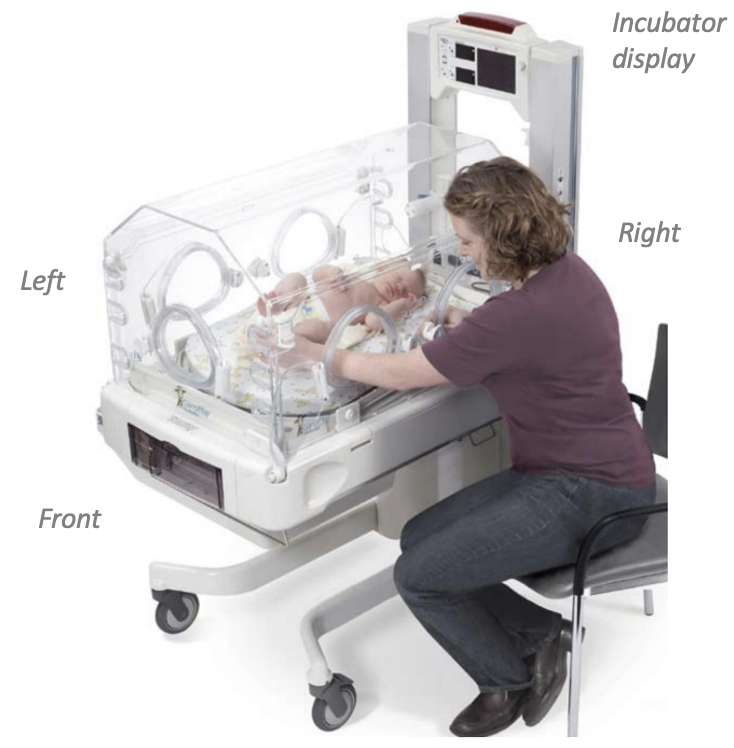
\includegraphics[width=0.5\textwidth]{Incubator Image.png}
    \caption{Image of the Giraffe Carestation CS1 provided by James Cook hospital \cite{Longanathan}.}
    \label{Fig 2.1:}
\end{figure}

\vspace{8mm}

\begin{figure}[H]
    \centering
    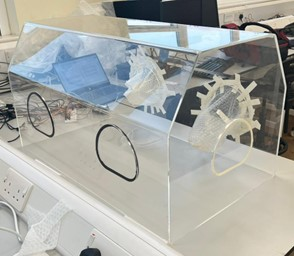
\includegraphics[width = 0.5\textwidth]{durhamModelPic.jpg}
    \captionsetup{justification=centering,margin=1cm}
    \caption{Photograph showing the model incubator in the Durham University laboratory. Electrical tape has been added to all of the porthole doors to better emulate the hospital incubator's insulation. The "sleeves" were then added after, for the improvements section.}
    \label{fig:durhamModelPic}
\end{figure}

The team used seven thermocouples in every experiment to measure the temperature at different positions inside the incubator. All of these were wired up to an Arduino (circuit board) which was connected to a laptop, and temperature readings were collected by running a code in Python (programming language) for 20 minutes. More information on the electronics setup can be found in section 11.1 (Arduino Circuit Diagrams) of the appendix. Fig. \ref{modelSketchPic} and Fig. \ref{hospitalModelPic} show the setup of the thermocouples in a diagram and in the hospital respectively. This setup was kept the same for all the experiments, including those done at the hospital and on the model incubator in Durham. Fig. \ref{Positioning of thermocouples} gives a written description of the positioning and purpose of each thermocouple.

\vspace{3mm}

\begin{figure}[h!]
    \centering
    \captionsetup{justification=centering,margin=1cm}
    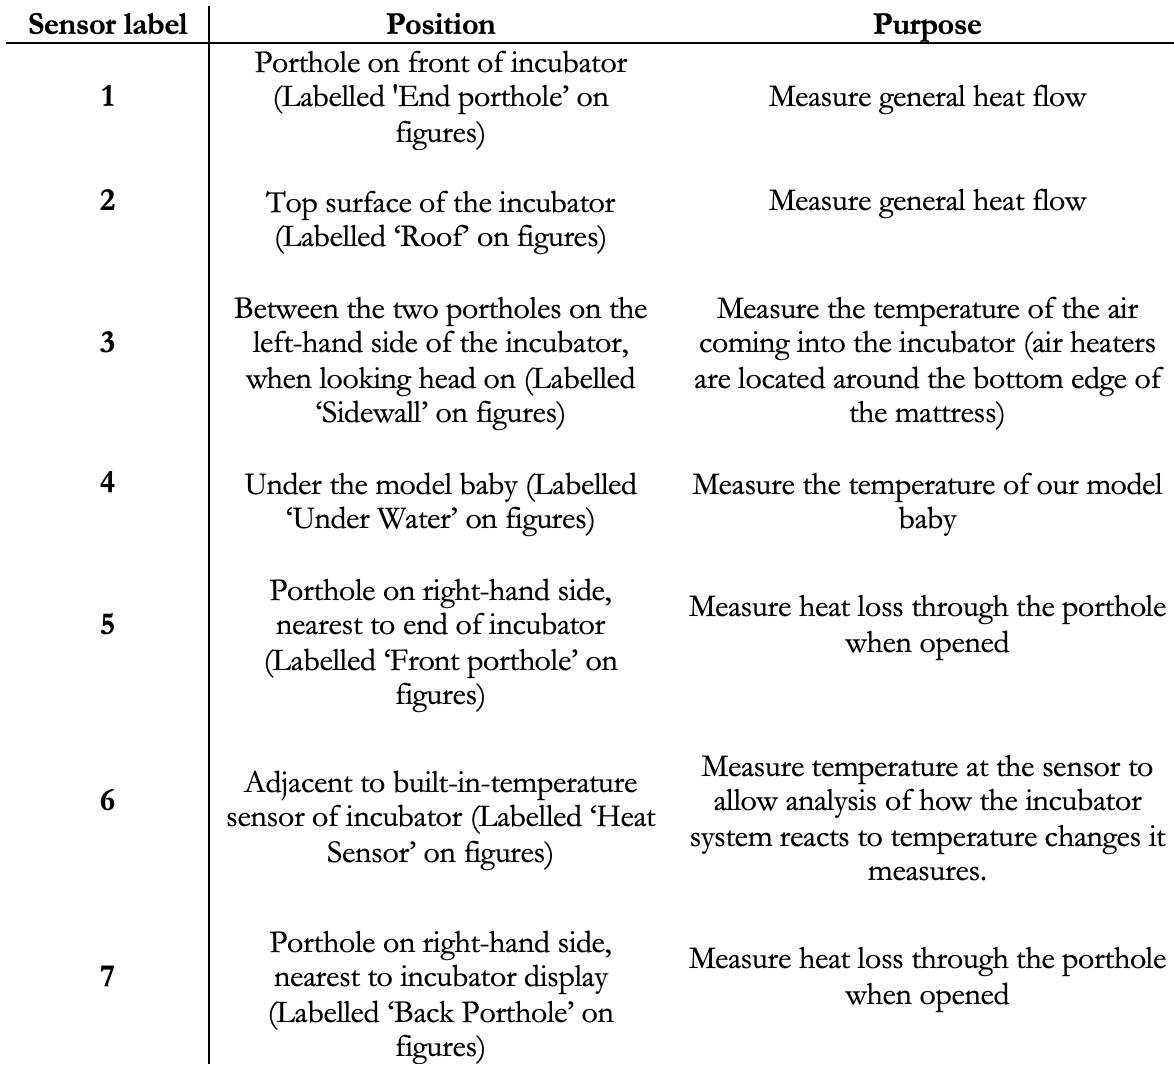
\includegraphics[width = 0.7\textwidth]{Positioning of thermocouples.png}
    \caption{Description of positioning and purpose of thermocouples inside the incubator.}
    \label{Positioning of thermocouples}
\end{figure}

\begin{figure}[h!]
\centering
\begin{minipage}{.45\linewidth}
    \captionsetup{justification=centering,margin=0.5cm}
    \centering{}
    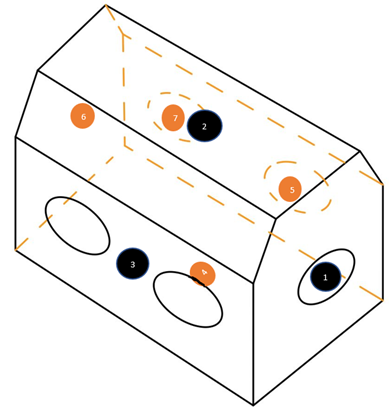
\includegraphics[width=0.7\textwidth]{modelSketchPic.png}
    \caption{Diagram showing thermocouple positions on the incubator.}
    \label{modelSketchPic}
\end{minipage}
\hfill
\begin{minipage}{.5\linewidth}
    \captionsetup{justification=centering,margin=0.3cm}
    \centering{}
    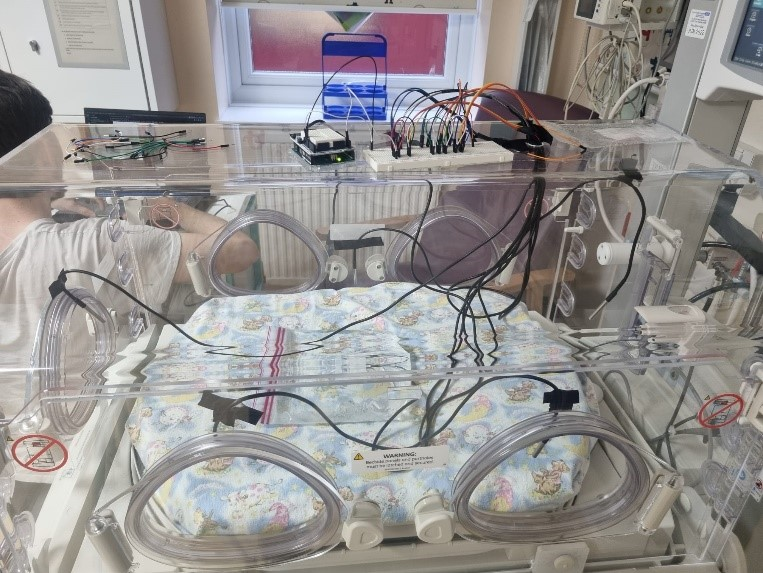
\includegraphics[width=0.7\textwidth]{hospitalModelPic.jpg}
    \caption{Photograph of the hospital incubator with thermocouples attached. The thermocouples are the silver parts on the end of the wires. All thermocouples are visible in the image apart from sensors 2 and 4 which are still in place but hidden due to the walls of the incubator.}
    \label{hospitalModelPic}
    \end{minipage}
\end{figure}


The decision to place sensor 4 beneath the model baby (freezer bag) was made because the bag usually had an air bubble at the top, therefore making it difficult to measure the temperature of the bag accurately from above. The team also made the assumption that because the incubator is symmetrical, there would not be a significant difference in heat loss between the right and left sides of the incubator when the portholes were opened, hence justifying the positioning of sensors 5 and 7 and the absence of sensors on the left-hand side portholes.

\vspace{3mm}

For all experiments, the team simulated a model baby by filling a freezer bag with approximately 1 kg of water. It was then placed on the middle of the mattress of the incubator for the duration of a measurement. For the experiments on air mode, air boost and on the model incubator in Durham, it was aimed for the initial temperature of the freezer bag to be 37°C, although this temperature was not controlled throughout experiments (see section 3 for more details). At the start of the experiments on servo mode, the temperature of the freezer bag was measured at 23°C, 35°C, and 40°C. This range was deliberately allowed to examine how servo mode reacts to different baby temperatures. The water temperature was controlled initially by adding water from hot and cold taps to achieve approximately the correct temperature, then leaving the bag in the incubator to get it up/down to exactly the right temperature. The mass of the water was measured using a scale and was between 0.995 kg to 1.005 kg for all experiments.

\vspace{3mm}


Throughout the majority of experiments in the hospital, it was aimed to control the humidity at 75\% using the incubator settings. In the physics laboratory, the same technology was not available and therefore humidity could not be controlled in the same way. Instead, a water bath of (nearly) boiling water was placed inside the model incubator. The temperature and volume of the bath was adjusted to achieve a humidity of roughly 75\% (target humidity). The humidity was measured using a humidity sensor and ranged between 65\% and 85\% during the trials in Durham except for the “no-sleeves” experiment where the humidity dropped to 37\% at the lowest point. In both hospital and university experiments, a humidity sensor was placed at each end of the incubator so the team could determine the difference in humidity across the incubator throughout. It’s important to note that although humidity was easy to control when the portholes were closed, opening of the portholes generally caused a rapid and uncontrollable decrease in humidity inside the incubator. However, the team was still able to use the measurements of humidity to make some conclusions on the relationship between humidity and heat transfer (discussed more later in the report). 

\vspace{3mm}

The temperature outside the incubator was controlled by doing the experiments in the same room of the hospital and the same room in the physics laboratories. Closing all windows and doors and keeping constant heating inside the room allowed the external temperature to be controlled at 26$^{\circ}$C in the hospital and 21$^{\circ}$C in Durham, measured on separate external thermometers. 

\vspace{3mm}

Many different experiments were conducted. The variables included the incubator that was used, the incubator mode, initial temperature of the “baby” (freezer bag), the porthole configuration and other factors as shown in Fig. \ref{fig:ExperimentsTable}. Preliminary trials were also conducted that are not included in Fig. \ref{fig:ExperimentsTable}.

\vspace{3mm}


\begin{figure}[H]
    \centering
    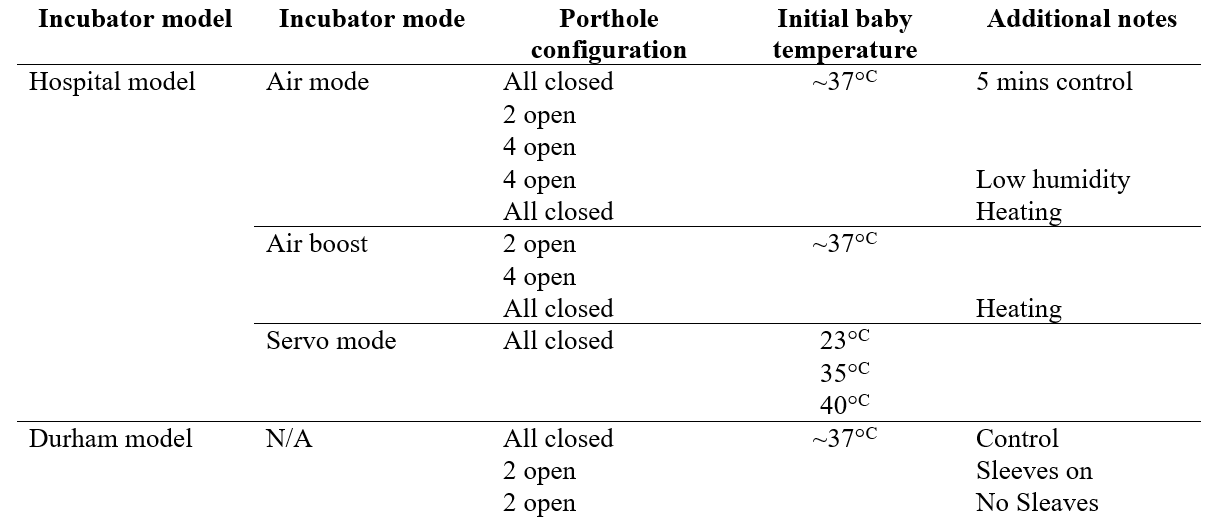
\includegraphics[scale = 0.5]{ExperimentsTable.png}
    \captionsetup{justification=centering,margin=1cm}
    \caption{Table showing the experiments conducted throughout the experiment.}
    \label{fig:ExperimentsTable}
\end{figure}



\vspace{3mm}

For experiments conducted with two portholes open, the open portholes were always on the “right-hand side” of the incubator. For experiments conducted with four open, the only closed porthole would be the porthole on the “front” of the incubator. Refer to Fig. \ref{Fig 2.1:} for reference to the porthole positions. More details on the experiments and additional notes can be found in later sections of the report. 



\begin{figure}[h!]
    \centering
    \captionsetup{justification=centering,margin=1cm}
    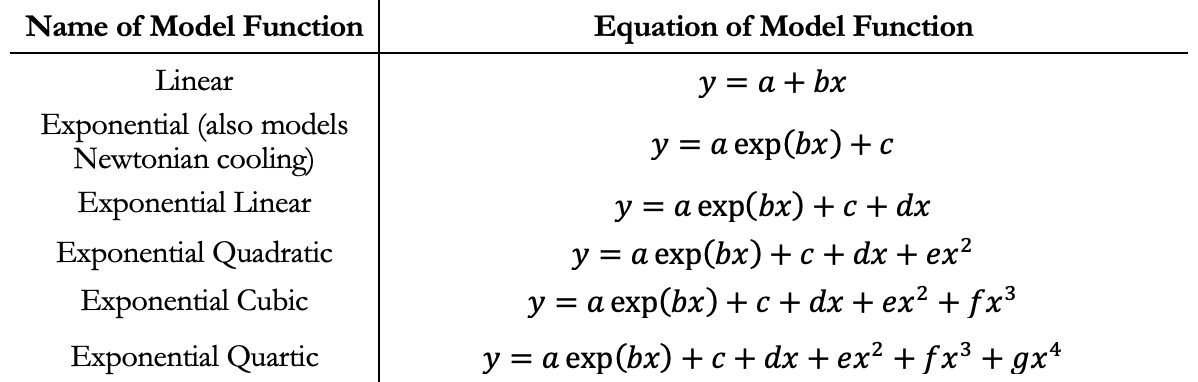
\includegraphics[width=0.8\textwidth]{Model functions table.png}
    \caption{List of all model functions that the measured data is fitted to using chi-squared analysis.}
    \label{ModelFunctTable}
\end{figure}

The data sets that the team obtained were fitted to various model functions using chi-squared analysis, all of which are shown in Fig. \ref{ModelFunctTable}.

\newpage
\section{Limitations}

Due to the nature of this team project, there have been several difficulties throughout that have impacted the progress of the team. Some of these difficulties have limited the project in certain ways and this subsection briefly describes those limitations and what the team has done to overcome them.

\vspace{3mm}

The most obvious difficulty with the project has been the distance between Durham and James Cook Hospital. With the drive to Middlesborough taking a minimum of forty-five minutes, it has not been possible for the team to travel to the hospital on a regular basis. As time at the hospital has therefore been limited, it has not been possible to conduct any repeat experiments and the team had to shorten the length of experiments to approximately 20 minutes per test. This is not ideal as the incubator doors could be open for periods of up to an hour in real practice, however the tests at the hospital showed that the temperature in the incubator tended towards a plateau after about 10 minutes, hence justifying the plan to do shorter experiments. The team also planned each hospital trip carefully to ensure that each individual would be completely prepared before arriving at the hospital and this allowed all the required measurements to be taken in the limited time. 

\vspace{3mm}

The team arranged for a model incubator to be made and sent to the laboratory in Durham so that measurements could be taken without travelling to Middlesborough. However, the model itself had its own limitations. The first issue was that the incubator took ten days longer to arrive than expected, which meant the team had to rearrange a hospital trip, change the order of experiments and limited the time with the model to only a week. Secondly, the incubator model was somewhat different to the actual incubator. Most significantly, the model did not have the different heating systems that are on the actual incubators. The systems are very intricate and expensive and therefore the team was unable to replicate aspects like servo mode or air boost mode. The team also had to add a heater and a humidifier to the laboratory model, which meant the system was inevitably different to that used at the hospital. Therefore, it was decided that all experiments conducted in Durham would be designed to test improvements. If a thermodynamic system is losing less heat due to an addition to the system, the addition is likely to cause improvements for the hospital incubator system too and therefore these tests were still valid. Other differences between the models include its lack of a “bed”, the absence of rubber material around the portholes and a slightly different plastic to the real incubator. However, these differences were relatively insignificant, especially after the experiments in Durham were changed to focus on testing improvements.

\vspace{3mm}

The final limitation of the project was the uncontrollable delays that the team experienced. One example of this was the first hospital trip, which was delayed by a week due to a miscommunication regarding transport. As the project was fixed within a time period of eight weeks, delays reduced the time that the team had to complete this project. As a result, the group had to be flexible with plans and had to make restrictions to the project and experiments such as those mentioned above. Ideally, the team would have taken more repeat measurements, improved the model of the incubator and conducted tests for longer periods, but the lack of time limited the team’s ability to do this and hence is the main reason why these improvements have not been made to the project.

\vspace{3mm}

\section{Air Mode \& Air Boost} \label{AirModeBoostSection}

\subsection{Introduction}
 \vspace{3mm}

Once a neonatal infant is deemed sufficiently thermally stable as to no longer require the use of ‘servo-mode', the baby is changed too ‘air mode’. This mode allows medical staff to set a desired temperature for the air by the use of a built-in temperature sensor positioned near the monitor and fixed in place within the incubator. The monitor allows for the setting of a specific target temperature. The primary downside to air mode is it doesn’t explicitly measure the baby’s temperature and relies on a general correlation between air temperature and the baby’s temperature. Hence, it is generally only used on neonates that have some level of independent thermal regulation. To test ‘air mode’, the temperature of the model baby (1kg of water) was measured, as well as the air temperature at 7 locations throughout incubator (as described in Sec. 4) to ascertain a causal relationship between the temperature of the model of the baby and the measurement provided by the inbuilt temperature sensor. 

 \vspace{3mm}

If portholes are required to be open for long periods of time, then it is common practise to use ‘air Boost’ or other equivalent mean of air propulsion in other incubators \cite{BTT10} . The function of ‘air Boost’ is to push hot air throughout the incubator to create a barrier, preventing heat escaping to the colder environment. Additionally, they can be used after the closure of incubator portholes to return the incubator to a specified temperature at a faster rate. The desired air temperature is input into the control monitor which then uses a temperature probe to periodically measure the temperature and adjust the heat and rate of flow of the air in line with this target. Interviews with medical staff in the NICU (neonatal intensive care unit) at The James Cook University Hospital revealed that common procedures such as installing central lines or cannulas could take anywhere up to 60 minutes in extreme cases but were likely to take approximately 20 minutes.  
\subsection{Air Mode - Additional Methodology}
\vspace{3mm}
‘Air mode’ was  tested under four conditions: 2 porthole doors open at high humidity(approximately 75 \%), 4 porthole doors open at high humidity (approximately 75 \%), 4 porthole doors open at low humidity(approximately 40 \%), and all doors closed. This was done to ascertain how effective ‘air mode’ was at maintaining temperature and humidity, and how variations in the level of humidity causes changes to the efficacy of reducing heat loss. 
\
\subsection{Air Mode - Results} \label{AirModeResults}
\vspace{3mm}
The relationship between the temperature of each thermocouple with increasing time period with various experimental configurations is shown in the figures below. Furthermore, the relationship between the humidity with evolving time period is shown below. Only the model functions are displayed to make graph look clearer without the data points. This decision was made as all the reduced chi-squared values were approximately equal to or less than 1, therefore suggesting the model function is a suitable fit to the data. 

\begin{figure}[H]
\centering
\begin{minipage}{0.57\linewidth}
    \captionsetup{justification=centering,margin=0.1cm}
    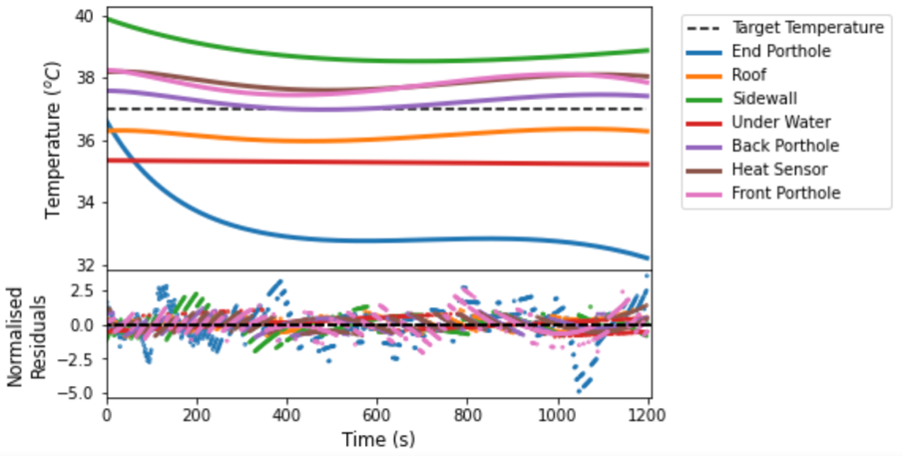
\includegraphics[width=\textwidth]{model functions 4 doors open.png}
    \caption{Plot of the model functions to display the relationship between the temperature with increasing time with 4 porthole doors open. \textit{Note: The plot of the temperature of the thermocouple at the heat sensor location is overlapped by the plot of the temperature of the thermocouple at the front porthole.}}
\end{minipage}
\hfill
\begin{minipage}{.42\linewidth}
    \captionsetup{justification=centering,margin=0.6cm}
    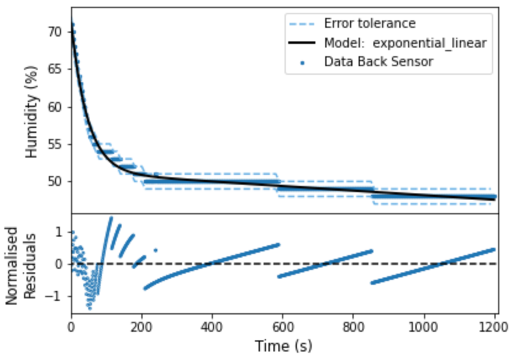
\includegraphics[width=\textwidth]{humidity 4 doors open.png}
    \caption{Relationship between the humidity with evolving time period with 4 porthole doors open. \textit{Note: The error bar limits are shown by the dashed line and too small to be seen in some areas.} }
    \end{minipage}
\end{figure}



\begin{figure}[H]
\centering
\begin{minipage}{.48\linewidth}
    \captionsetup{justification=centering,margin=0.5cm}
    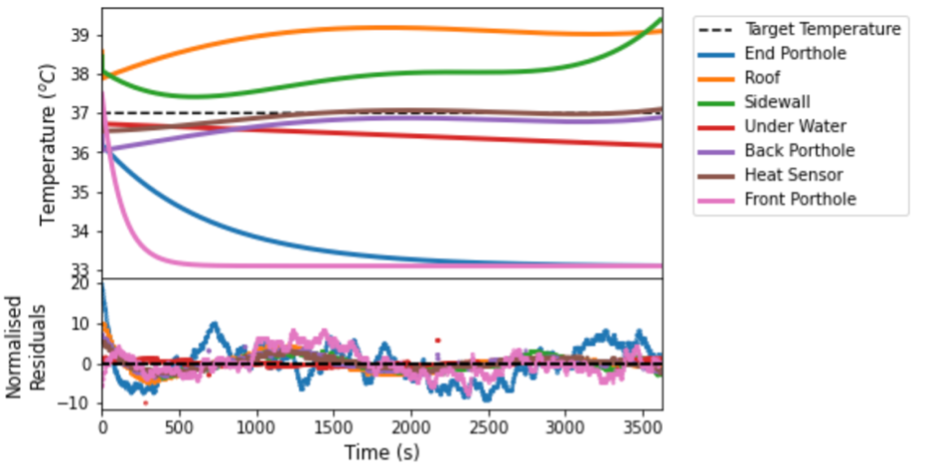
\includegraphics[width=\textwidth]{4 doors open low humidity.png}
    \caption{Plot of the model functions to display the relationship between the temperature with increasing time with a low humidity setting ranging between (24 $\pm$ 1) $\%$ to (29 $\pm$ 1) $\%$ with 4 porthole doors open.}
\end{minipage}
\hfill
\begin{minipage}{.48\linewidth}
    \captionsetup{justification=centering}
    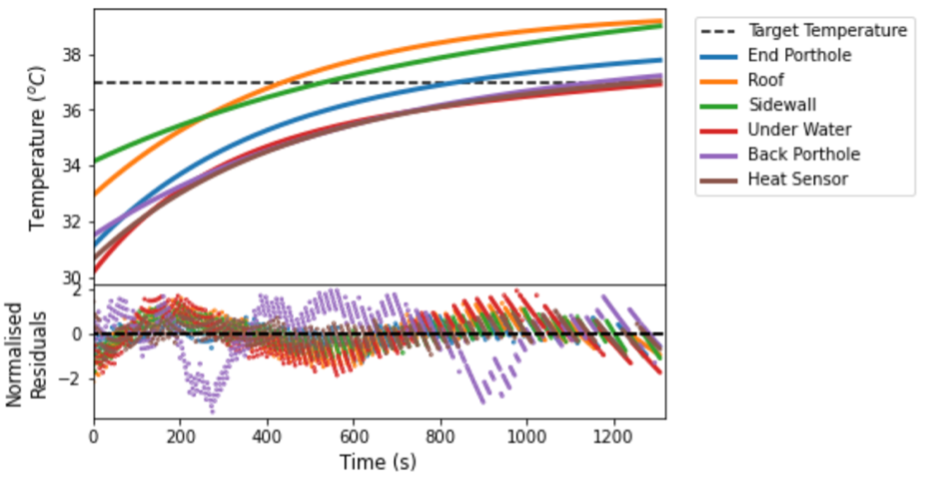
\includegraphics[width=\textwidth]{temperature increasing.png}
    \caption{Relationship between the temperature of the thermocouples with increasing time with all porthole doors closed starting from a low temperature. \textit{Note: The model function for the underwater thermocouple and heat sensor thermocouple are overlapped and hence not visible.}}
    \end{minipage}
\end{figure}



\begin{figure}[H]
\centering
\begin{minipage}{.43\linewidth}
    \captionsetup{justification=centering,margin=0.5cm}
    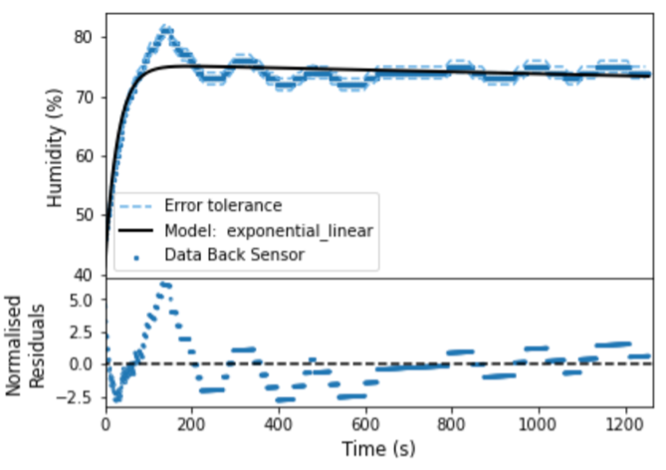
\includegraphics[width=\textwidth]{Humidity increase.png}
    \caption{Relationship between the humidity with evolving time with all porthole doors closed. \textit{Note: The error bar limits are shown by a dashed line, which may be too small to be seen in some areas.}}
\end{minipage}
\hfill
\begin{minipage}{.56\linewidth}
    \captionsetup{justification=centering,margin=0.1cm}
    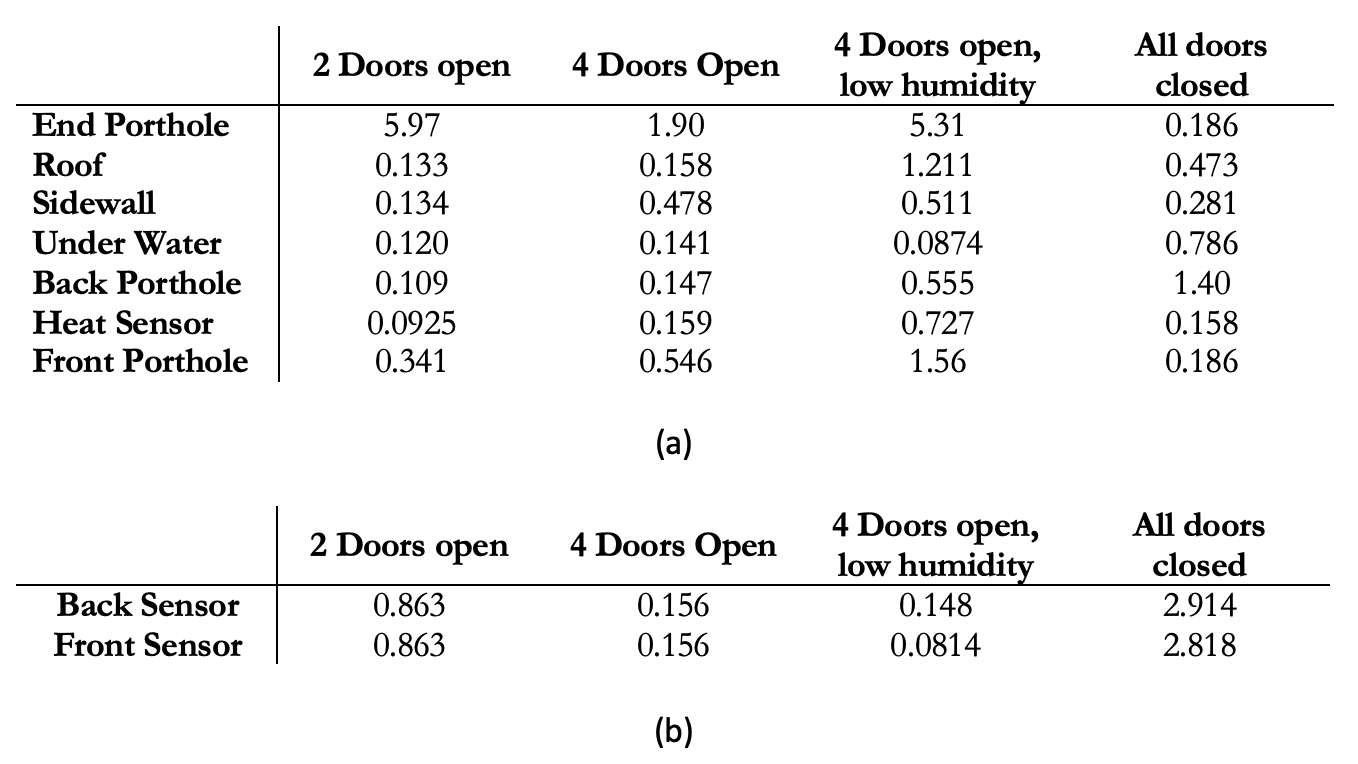
\includegraphics[width=\textwidth]{Air mode table.png}
    \caption{Reduced chi-squared values for; (a) Each thermocouple after chi-squared analysis to individual model functions, (b) for each humidity sensor after chi-squared analysis to the exponential linear model function.}
    \end{minipage}
\end{figure}

\subsection{Air Mode - Discussion} \label{AirModeDiscussion}
\vspace{3mm}
As shown in Fig. 6.1, although 4 porthole doors were open, the temperature at the front and back porthole remain one of the highest amongst the other thermocouples. This may be due to the built-in heater being located around the perimeter of the mattress inside the incubator, which is directly below the portholes. Therefore, the temperature from the front and back thermocouples suggests the temperature readings are heavily influenced by the temperature of the air coming out from the heater. Therefore, it was not possible to measure accurately how much heat is lost through the portholes.

\vspace{3mm}

Although the most significant location of heat loss is at the end of the incubator, the temperature around other areas of the incubator remain in a narrow range as shown in Fig. 6.1. The rear may have had more heat loss due to small gaps in the housing of the incubator to allow for wire connections used by the hospital. However, a significant problem to the heat flow of the incubator is displayed by the thermocouple located under the bag of water, corresponding to the model of the baby, shown in Fig. 6.1. The temperature of the thermocouple placed below the baby model drops from a maximum value of (35.59 $\pm$ $0.06) ^{\circ}$C to a minimum of (35.50 $\pm$ 0.06 )$^{\circ}$C  at a rate of (-1.03 $\pm$ 0.06)  \times10$^{-4}^{\circ}$Cs$^{-1}$ when 4 doors are open. Although the temperature drop was negligible, these temperatures pose a significant risk to hypothermia for a premature baby. 

\vspace{3mm}

Furthermore in Fig. 6.1, the difference between the temperature of the thermocouple at the baby model and the heat sensor of the incubator ranges by approximately 3 $^{\circ}$C. Therefore, even if the temperature of the baby is at a critical temperature, the incubator is unable to recognise this threat. As shown by the thermocouple at the sidewall, the temperature of the air coming out of the heater slowly drops as the incubator system believes it has reached the target temperature by its temperature sensor reading.

\vspace{3mm}

As shown in Fig. 6.2, the humidity with 4 porthole doors open rapidly falls to approximately 50 \% within the first 3 minutes of the opening of the portholes. The air from the heater may cause the humidity to be lost faster as they are located directly beneath the porthole openings, encouraging more air to flow out through these doors. 

\vspace{3mm}

The same experiment of having 4 doors open but with a low humidity setting was conducted to explore the impact of humidity on the heat loss shown in Fig. 6.3. Comparing the results between Fig. 6.1 and Fig. 6.3, the temperature at the roof of the incubator is higher at a lower humidity setting than at a higher humidity setting. This suggests the heat flow out through the portholes is less significant at a lower humidity and the hot air from the heater is able to contribute more to the convection currents. 

\vspace{3mm}

However, the thermocouple at the front porthole shows it is one of the most significant sources of heat loss as shown in Fig. 6.3. Despite 4 portholes being open, the temperature at the back porthole continues to increase. Furthermore, similarly with Fig. 6.1, the end porthole remains to be a significant source of heat loss. The difference in temperature between the end and back porthole suggests the temperature of the air from the heater is higher for the heater locations below the front and back portholes than the portholes at the end of the incubator. This is likely due to the how the incubator system is programmed; as the portholes at the front and back porthole is more likely to be opened than at the end porthole, the heater allows for more heat loss through these locations, therefore increasing the air temperature. 

\vspace{3mm}

The discrepancy between the temperature data sets of the front porthole in Fig. 6.1 and Fig. 6.3 is likely due to a slight difference in experimental set up. The front porthole thermocouple in Fig. 6.1 may have been slightly lower than when conducting the experiment in Fig. 6.3, therefore, the temperature of the air from the heater having more influence over the temperature readings. An alternative explanation may be due to the location of the humidifier in the incubators. If they are located at the end of the incubator, the hot air from the humidifier could have significantly affected the temperature of the thermocouple at the front porthole in Fig. 6.1. However, at a low humidity, due to the lack of water in the humidifier, there is less hot air coming from the end of the incubator, causing a lower temperature at the front porthole in Fig. 6.3.

\vspace{3mm}

As shown in Fig. 6.3, the rate of temperature decrease of the baby model was linear, however was negligible with a rate of $(-1.53 \pm 0.01) \times 10 ^{-4}^{\circ}$C$s^{-1}$. The range of the temperatures of thermocouple at the model of the baby was less than 0.2 $^{\circ}$C. As mentioned previously, the rate of temperature decrease at a high humidity was also negligible at a rate of (1.03 \pm 0.06) \times 10 $^{-3}$ $^{\circ}$Cs$^{-1}$. When comparing these rates, the rate of temperature decrease at a low humidity was 49 \% higher than at a higher humidity. However, as both these rates are negligible, the rate of heat loss for different humidity levels does not have a significant impact on the temperature of the baby.

\vspace{3mm}

Furthermore, the temperature of the air from the heater, shown by the thermocouple on the sidewall, is higher than the target temperature and increases even if the temperature of the heat sensor reaches the target temperature as shown in Fig. 6.3. Therefore, this suggests 'air mode' allows for heat loss during air circulation by aiming to achieve a higher temperature at the heat sensor than the set target temperature.

\vspace{3mm}

Fig. 6.4 shows how fast the incubator can reach the target temperature when starting from a low temperature with all doors closed. The humidity readings for the same experiment are shown in Fig. 6.5. The humidity recovers at a fast rate, reaching the desired percentage after approximately only one minute. The rate at which the temperature increases at various locations through the incubator is similar, and the time taken for the baby model to start at 35 $^{\circ}$C and reach 37 $^{\circ}$C is approximately 12 minutes. Therefore, in critical conditions, air boost may be used in preference to reach the desired temperature at a faster rate. 

\subsection{Air Boost - Additional Methodology}

\vspace{3mm}



Measurements of temperature and humidity were taken for 20 minutes with three different porthole configurations (2 portholes on the same side open, all 4 side portholes open, and all portholes closed after recovering from low air temperature [30°C]) This was done to measure the efficacy of 'air boost' as a means of preventing heat loss and recovering heat within the incubator after long exposures to ambient temperature. 

\subsection{Air Boost - Results}

The measured temperatures at various incubator locations over a time period of roughly 20 minutes are shown in the figures below. Results are plotted for various experimental setups, each with different porthole configurations. Additionally, humidity data is shown plotted against time from two humidity sensors over two experimental setups. In all figures below, only the model functions are shown for ease of interpretation. This decision was justified as all the chi-squared values associated with the data were roughly equal to or less than 1, therefore the models were a good fit to the data. 

\vspace{3mm}


\begin{figure}[H]
\centering
\begin{minipage}{.57\linewidth}
    \captionsetup{justification=centering,margin=0.5cm}
    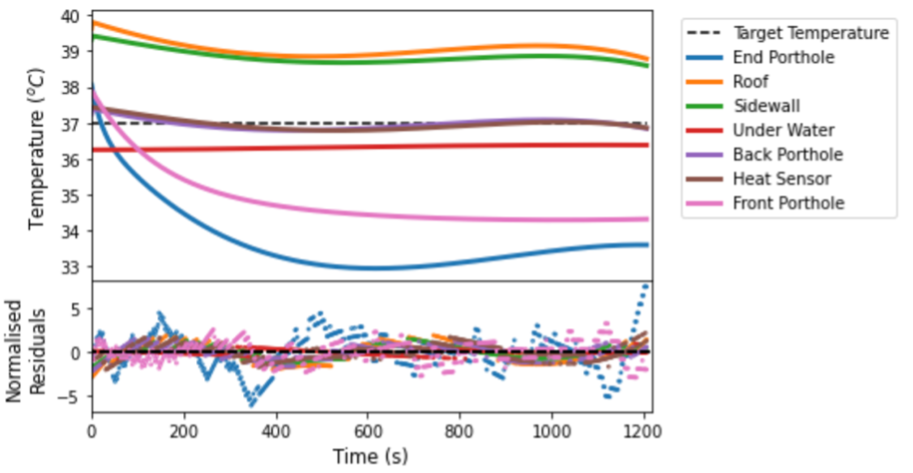
\includegraphics[width=\textwidth]{Two holes air boost.png}
    \caption{Temperature variation with time at various temperature probe locations. Two portholes were open and 'air boost’ was enabled. \textit{Note: The lines for heat sensor and back porthole are overlapped.}}
\end{minipage}
\hfill
\begin{minipage}{.42\linewidth}
    \captionsetup{justification=centering,margin=0.3cm}
    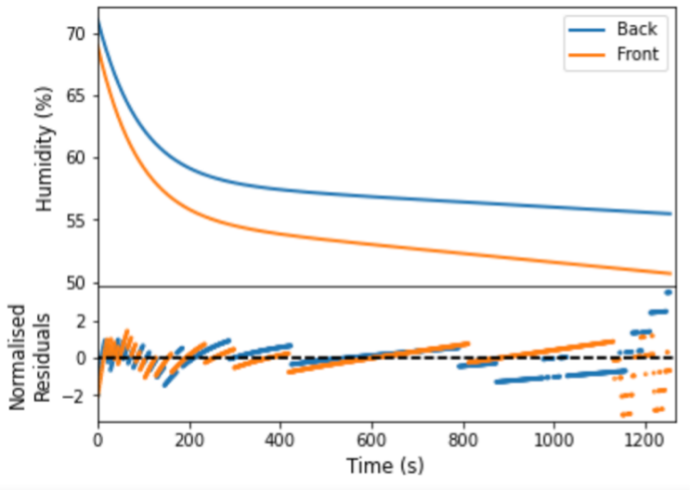
\includegraphics[width=\textwidth]{two door humidity air boost.png}
    \caption{Humidity variation with time at two locations inside the incubator. Two portholes were open and 'air boost' was enabled.}
    \end{minipage}
\end{figure}



\begin{figure}[H]
\centering
\begin{minipage}{.57\linewidth}
    \captionsetup{justification=centering,margin=0.5cm}
    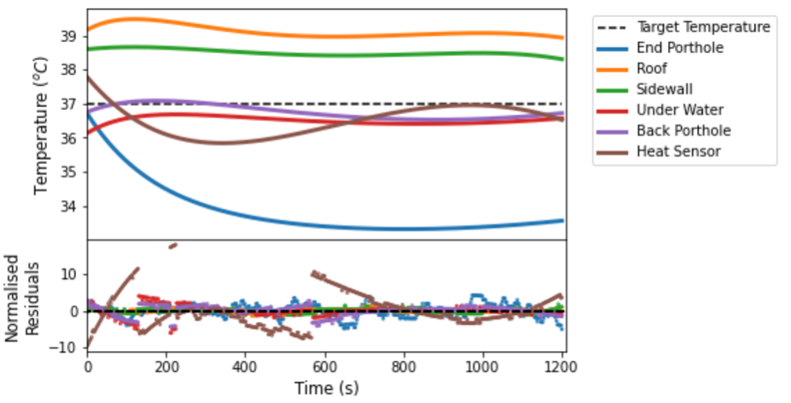
\includegraphics[width=\textwidth]{4 holes air boost.png}
    \caption{Temperature variation with time at various temperature probe locations. Four portholes were open and 'air boost' was enabled.}
\end{minipage}
\hfill
\begin{minipage}{.42\linewidth}
    \captionsetup{justification=centering,margin=0.3cm}
    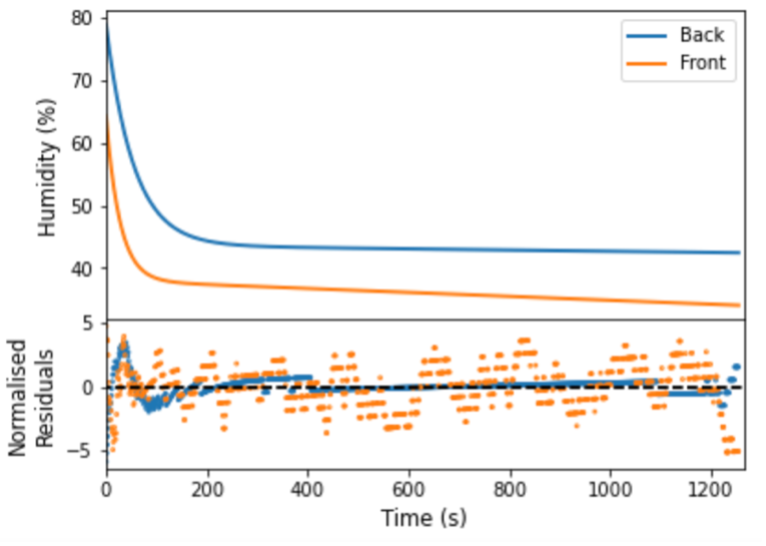
\includegraphics[width=\textwidth]{4 doors humidity air boost.png}
    \caption{Humidity variation with time at two locations inside the incubator. Four portholes were open and 'air boost' was enabled.}
    \end{minipage}
\end{figure}



\begin{figure}[H]
\centering
\begin{minipage}{.57\linewidth}
    \captionsetup{justification=centering,margin=0.7cm}
    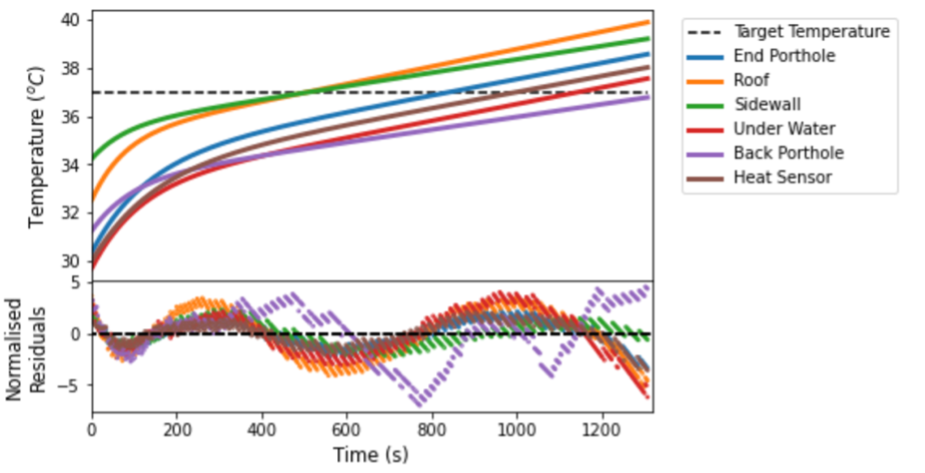
\includegraphics[width=\textwidth]{closed air boost.png}
    \caption{A graph showing temperature variation with time at various thermocouples when trying to heat the incubator up from cool. All portholes were closed, and 'air boost' was enabled.}
\end{minipage}
\hfill
\begin{minipage}{.42\linewidth}
    \captionsetup{justification=centering,margin=0.1cm}
    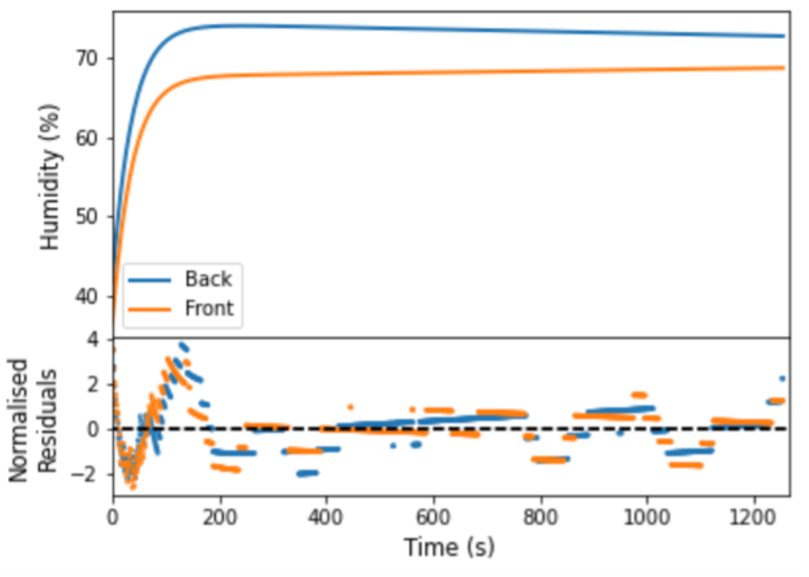
\includegraphics[width=0.95\textwidth]{Humidity air boost cl;osed.png}
    \caption{A graph showing increasing humidity with time for two humidity sensors at the front and back of the incubator, while trying to heat the incubator up from cool. All portholes were closed and 'Air boost' was enabled.}
    \end{minipage}
\end{figure}

\subsection{Air Boost - Discussion}

As shown in Fig. 6.7, the temperature underneath the water remained constant (within 0.5$^{\circ}$C) throughout the period of data taking. This result proved promising as it suggested that the underside of a baby would remain well within a safe body temperature \cite{JG4} range during a two-porthole-open procedure. Concerning, however, there was a discrepancy of up to roughly 1.5 $^{\circ}$C between the under-water sensor and the incubator’s own heat sensor. This difference was seen in 'Air mode' as well (see Sec. \ref{AirModeResults}). This discrepancy once again suggested the incubator could have been inaccurately measuring the temperature the baby exhibited  and make disproportionate adjustments, however it could also be indicative of variations in the position of the placement of temperature sensors.

  \vspace{3mm}

Fig 6.7 illustrates a significant drop in temperature near Front Porthole, reaching temperatures approaching 34$^{\circ}$C. This is mimicked by the temperature drop at end Porthole, hitting temperatures lower than 33$^{\circ}$C suggesting the area of most dramatic heat loss is near the baby’s head. If the baby’s head is sitting in an environment of critically low temperature, even without the end porthole open, there could be serious medical consequences. 

  \vspace{3mm}

Fig 6.7, reassuringly, aligns with expectations, showing that temperature remains consistently high (39$^{\circ}$C - 40$^{\circ}$C) at the roof (consistent with expectations due to the principle of hot air preferentially rising) and right above the heaters (where the outputted hot air has not yet had chance to cool). 

  \vspace{3mm}

Fig 6.9 shows temperature variation with time with 'air boost' on and four portholes open. This data tells much the same story as having two doors open, however with more significant drops in temperature and more fluctuations. For example, the baby temperature remains around its initial value, however sees an almost sinusoidal fluctuation over the course of 1200 seconds. This behaviour is seen in the back Porthole and heat sensor data, too. The roof and sidewall temperatures remain the highest, like before, however now sit at a temperature 1$^{\circ}$C - 2$^{\circ}$C lower than the two-porthole-open experiment. 

  \vspace{3mm}

Fig 6.11 shows how quickly the incubator is able to get up to temperature after starting quite low. The heating process appears to occur in two stages: initially, the temperature rises steeply, with all thermocouples experiencing a rapid, linear rise in temperature. Subsequently, after roughly 200 seconds, the rate of temperature increase at all thermocouple locations decreases, then rising steadily in an almost linear fashion. The rate of humidity increase, Fig 6.12, is approximately the same as that of 'air mode', which is consistent with expectations as both sets of data involved no open doors and hence no way for moisture to escape. Fig 6.12 suggests the humidity increases at a greater rate at the back of the incubator, potentially due to the location of the humidifier. Fig 6.12 also suggests that the front and back humidity values will converge at large time values and approach the set value inputted in the incubator’s display. 


\subsection{Comparison between Air Mode and Air Boost} \label{ModeBoostComparison}

For both data sets ('air boost' and 'air mode'), the most significant source of heat loss and humidity loss was observed at the end of the incubator (see Fig. 6.7 and Fig. 6.9). The end Porthole thermocouple in Fig. 5.7 measured a minimum temperature of just below 33$^{\circ}$C – a minimum that is nearly 2$^{\circ}$C lower than the next lowest thermocouple minimum (that being Front Porthole). The temperature of the roof of the incubator and at the incubator’s heat sensor was measured to be higher when using ‘Air boost’ mode. This result suggests that there is less air lost through the portholes and instead more air contributing to the convection currents through the incubator. With four portholes open (Fig. 6.1 and Fig. 6.9), neither ‘Air mode’ nor ‘Air boost’ raised the model baby temperature to the target level that was set. Both settings, however, did maintain the baby’s temperature to some extent - Fig. 6.1 shows a low-rate temperature decrease (addressed in Sec. \ref{AirModeDiscussion}) during ‘Air mode’ and Fig. 6.9 (‘Air boost’ enabled for the same porthole configuration) shows +/- 0.5$^{\circ}$C fluctuations, but no evidence of temperature overall trending downwards with time within the data taking period. As such, one might conclude that ‘Air mode’ and ‘Air boost’ are both effective at maintaining baby temperature while portholes are open, however not effective at raising baby temperature in such scenarios. 

  \vspace{3mm}


The minimum humidity level in the incubator is lower when using the ‘Air boost’ setting than the 'Air mode' setting – 47\% during ‘Air mode’ and 43\% during ‘Air boost’ for the Back humidity sensor (see Figures 6.2 and 6.10). Humidity is closely related to a system’s ability to retain heat (see Sec. \ref{Thermodynamic}) and as such, one might expect a lower-humidity system to lose heat faster. However, the minimum temperature reached is lower using the 'Air mode' setting – the higher humidity case - hitting 36.5$^{\circ}$C in ‘Air mode’ and 37.5$^{\circ}$C in ‘Air boost’ mode for the Heat Sensor thermocouple. One might conclude from this that despite Air boost’s tendency to dry out the air in the system, the rapid pace at which it adds heat counteracts this to prevent temperatures dropping so drastically.  

  \vspace{3mm}


Figures 6.4 and 6.11 (‘air mode’ and ‘air boost,’ respectively) show temperature change (at various thermocouple locations throughout the 20-minute data-taking window) while the incubator was heating up from a low-temperature starting point. Comparing the two figures, ‘air boost’ exhibited a higher rate of temperature increase at the start of the time window (0-200 s) before then adopting a lower, linear rate of temperature increase for the remaining time, whereas ‘Air mode’ resembled more of a sloping curve of decreasing gradient. Looking at the under water sensor (the sensor placed underneath our model baby, the 1 kg bag of water), it took ‘air mode’ 12 minutes to raise the temperature from 35$^{\circ}$C to 37$^{\circ}$C, whereas ‘air boost’ only took 10 minutes to perform the same heating interval. Therefore, ‘air boost’ is better for heating a low-temperature baby and incubator as it reaches the desired temperature faster. 

  \vspace{3mm}


Interestingly, Fig. 6.4 suggests the temperature the baby would experience (under water thermocouple) will tend towards the target temperature in ‘air mode’ - that is to say the temperature levels-off such that it settles on 37$^{\circ}$C. Differently, however, in ‘air boost’ mode, the linear increase in temperature for the under water sensor (and all sensors for that matter) appears to continue beyond the target temperature (see Fig. 6.11), reaching a temperature of approximately 37.5$^{\circ}$C without any signs of slowing. It is impossible to describe the way in which the temperature will behave beyond the window of our data taking as the incubator might action changes to regulate the temperature after this over-shooting, however one can expect more increase before any changes come into effect. This prediction could imply excessively high incubator and new-born temperatures.  


\section{Servo mode}
\subsection{Introduction}
\vspace{3mm}
As previously mentioned, the second ‘mode’ built into the incubator is the Servo/Baby mode. This is generally used in the first 2 weeks of life. Due to the large surface area to volume ratio of a prenatal baby, and the lack of subcutaneous fat causing weak insulation, rapid heat loss can occur unexpectedly. The purpose of this mode is to precisely measure the temperature of the baby constantly to detect any sudden changes in the temperature of the baby, so the system can then automatically adjust the temperature of the incubator accordingly. The nurse responsible for the baby will set a ‘target’ temperature using the screen on the incubator which acts as the target for the baby’s temperature, not the air temperature. Through a live feed from the thermocouple attached to the baby, the incubator's computer system adjusts the air temperature \cite{LS1}. For example, if the baby’s temperature dropped to 36$^{\circ}$C (below the average set temperature of 37$^{\circ}$C) then the incubator responds by increasing the air temperature to boost the baby’s temperature back to normal levels. 
 
 \vspace{3mm}
 
The nurses at the hospital noted their opinions of servo mode. Their concern was that if a baby’s temperature dropped by, say, 0.5$^{\circ}$C the system would increase the temperature by 2$^{\circ}$C, which would be too much and could cause harm to the baby. The other issue was with how the thermocouple attaches to the baby. Currently, a sticker is used which is applied over the thermocouple onto the baby’s skin. A neonatal baby’s skin is extremely fragile, and the sticker can cause damage to the skin. Another problem is that the incubator is hot and humid causing the sticker to sometimes fall off or move meaning the temperature of the baby is measured lower than it should be. This causes the incubator to increase its temperature even if the baby is at an ideal temperature. Both issues are to be addressed in the experiments. 
 
 \vspace{3mm}
 
The question at hand refers to exactly how the servo mode responds to changes in the baby’s skin temperature. How long it takes to boost the air temperature and by how many degrees, or conversely how the temperature is reduced for an overheating baby, were the primary problems to understand.

\subsection{Additional Methodology}
\vspace{3mm}
The technical set-up in regards to the positioning of the thermocouples and humidity sensors was exactly the same as with air mode. The humidity was set to 75\% and the ‘target’ baby temperature to 37$^{\circ}$C, due to the advice given by hospital staff. A baby was modelled as a 1kg bag of water. A mix of hot and cold water was used to achieve a model baby of desired temperature, and checked with a thermal probe. The probe that usually connects to the baby was then attached to the bag of water to give a representation of the temperature of the baby. The experiment was run over 20 minutes for 3 different water temperatures chosen to be 23$^{\circ}$C, 35$^{\circ}$C, and 40$^{\circ}$C, each with a respective uncertainty of $\pm$ 0.1$^{\circ}$C. The port holes were all shut for this experiment.

\subsection{Results}
 \vspace{3mm}
All error analyses can be found in the appendix (Sec. 11.2).
The ambient temperature for the room was found to be 26 $\pm$ 0.1$^{\circ}$C. This was measured as a control so that our experiments had the same heat differential to the surroundings throughout. The Servo mode was tested at three different baby temperatures and data was collected via the python code for 6 different thermocouples located around the incubator. 


\vspace{3mm}

Please refer to the Methodology (Sec. 4), for definitions of the models that the data has been tested against. The target temperature was also included in graphs where applicable. Some graphs have been selected and can be seen below. 


\begin{figure}[H]
\centering
\begin{minipage}{.48\linewidth}
    \captionsetup{justification=centering,margin=0.3cm}
    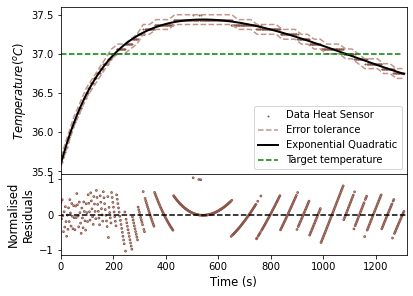
\includegraphics[width=\linewidth]{Heat sensor 40C.png}
    \caption{The plot of the heat sensor thermocouple for a baby at 40$^{\circ}$C, with the normalised residual below. \textit{Note: Errors have been plotted as ‘bands’ outlined by the dashed lines}.}
    \label{40C HS}
\end{minipage}
\hfill
\begin{minipage}{.48\linewidth}
    \captionsetup{justification=centering,margin=0.6cm}
    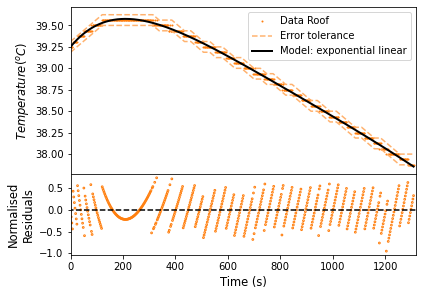
\includegraphics[width=\linewidth]{Roof 40C.png}
    \caption{The plot of the roof thermocouple for a baby at 40$^{\circ}$C, with the normalised residual below. \textit{Note: Errors have been plotted as ‘bands’ outlined by the dashed lines}.}
    \label{40C roof}
    \end{minipage}
\end{figure}


\begin{figure}[H]
\centering
\begin{minipage}{.48\linewidth}
    \captionsetup{justification=centering,margin=0.3cm}
    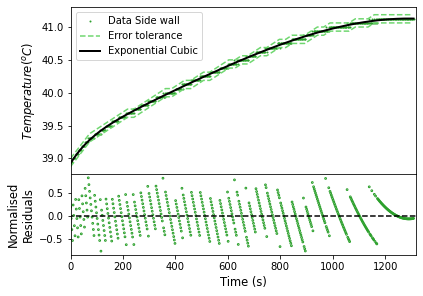
\includegraphics[width=\linewidth]{Side wall 35C.png}
    \caption{The plot of the side wall thermocouple for a baby at 35$^{\circ}$C, with the normalised residual below. \textit{Note: Errors have been plotted as ‘bands’ outlined by the dashed lines}.}
    \label{35C SW}
\end{minipage}
\hfill
\begin{minipage}{.48\linewidth}
    \captionsetup{justification=centering,margin=0.3cm}
    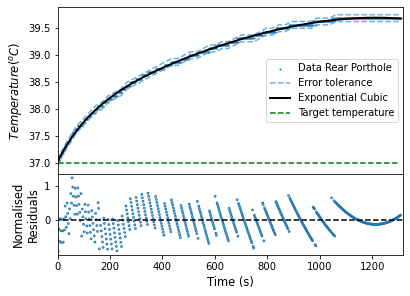
\includegraphics[width=0.99\linewidth]{Rear 35C.png}
    \caption{The plot of the rear porthole thermocouple for a baby at 35$^{\circ}$C, with the normalised residual below. \textit{Note: Errors have been plotted as ‘bands’ outlined by the dashed lines}.}
    \label{35C Rear}
    \end{minipage}
\end{figure}


\begin{figure}[H]
\centering
\begin{minipage}{.48\linewidth}
    \captionsetup{justification=centering,margin=0.3cm}
    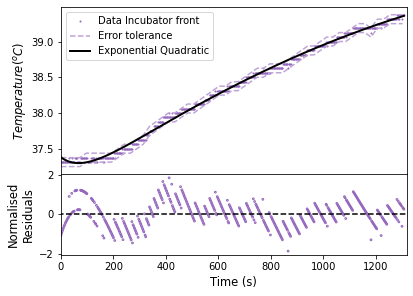
\includegraphics[width=\linewidth]{Incubator front 23C.png}
    \caption{The plot of the incubator front thermocouple for a baby at 23$^{\circ}$C, with the normalised residual below. \textit{Note: Errors have been plotted as ‘bands’ outlined by the dashed lines}.}
    \label{23C FRONT}
\end{minipage}
\hfill
\begin{minipage}{.48\linewidth}
    \captionsetup{justification=centering,margin=0.3 cm}
    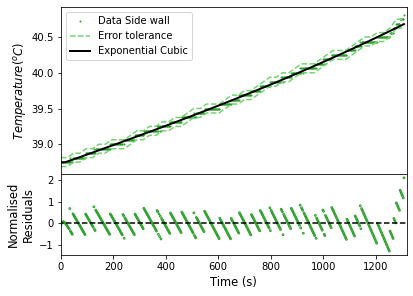
\includegraphics[width=\linewidth]{Side wall 23C.png}
    \caption{The plot of the side wall thermocouple for a baby at 23$^{\circ}$C, with the normalised residual below. \textit{Note: Errors have been plotted as ‘bands’ outlined by the dashed lines}.}
    \label{23C SW}
    \end{minipage}
\end{figure}

The top two graphs, Fig. \ref{40C HS} and Fig. 7.2,  show the temperature change for the roof and heat sensor locations for a baby at 40$^{\circ}$C. The overall trend was an exponential cubic. The middle graphs, Fig. \ref{35C SW} and Fig. \ref{35C Rear}, show the temperature change for the rear porthole and side wall locations for a baby at 35$^{\circ}$C. Again, the overall trend was an exponential cubic graph. The final two graphs, Fig. \ref{23C FRONT} and Fig. \ref{23C SW}, show the temperature change for the roof and the incubator front locations for a baby at 23$^{\circ}$C. The overall trend was an exponential quadratic.

\vspace{3mm}

Below shows the average parameter values in accordance with their respective best-fit model. The table below shows a representation of all the data for all 3 different experiments.

\begin{figure}[!h]
    \centering
    \captionsetup{justification=centering,margin=1cm}
    \includegraphics[width=0.95\textwidth]{Table Servo.png}
    \caption{A table with all the parameter values for the 3 different temperatures of baby, along with associated uncertainties. Values for reduced chi-square $\chi^{2}_{v}$ and $P(\chi^{2}_{min};v)$ are also recorded.}
    \label{Table servo}
\end{figure}

The humidity was also recorded in two separate locations of the incubator. As expected, due to the portholes being shut, the humidity remained constant around the 75\% that was set. Small fluctuations of 1\% occurred throughout the experiment. Therefore, the results have not been presented.

\subsection{Discussion}
\vspace{3mm}
Looking at the results there are several conclusions from the data. Studying the data, in Fig. \ref{Table servo}, for 40$^{\circ}$C the exponential parameter, b, is insignificant, as it is very small giving an exponential term equal to 1. This meant the driver of the temperature change came from the polynomial term. The terms are small, but it can be concluded that the temperature decreases as expected due to parameter values being negative. The general trend was a gradual increase, this is most likely due to the portholes just being closed causing the temperature inside to be lower than expected, followed by a decrease. Also the rate of this temperature decrease grew over time. The maximum temperature was recorded at around 350 seconds ($\approx$ 6min) after the portholes were closed. It was noted that it was difficult to decrease the temperature rapidly and this was shown in the average temperature difference between the maximum and minimum temperatures recorded over the 20 minutes to be just 1.53 $\pm$ 0.2$^{\circ}$C. 
 
 \vspace{3mm}
 
Studying the data for 35$^{\circ}$C the exponential term, b, is more significant (order of 10 bigger than in the 40$^{\circ}$C case). This means the temperature change depends on both the cubic term and the exponential function. Parameters d and e are both positive and since the parameter values are small, the sign of the parameters can be used to determine how the temperature changed over the period. Since these are both positive, it shows that the temperature increased as expected, but due to the negative cubic term and exponential term this rate of temperature increase slowed over time. All 6 plots showed that the incubator increased its temperature over the experimental time and came towards a peak at around 20 minutes. The average temperature change of the 6 thermocouples was 1.92 $\pm$ 0.2$^{\circ}$C. Comparing the different temperature changes for the 40$^{\circ}$C and the 35$^{\circ}$C baby shows that the incubators find it much easier to increase their temperature than decrease it. This is shown by the larger magnitude of parameter values showing a more aggressive temperature change in the 35$^{\circ}$C baby case. Since they were 3$^{\circ}$C and 2$^{\circ}$C different from the set temperature respectively, the data proves that temperature increase is easier for the incubator as it would be expected that there was a similar response to baby temperatures that are a similar differences from the set temperature. This data has proved this to be an incorrect hypothesis. 

\vspace{3mm}

Finally, the 23$^{\circ}$C data showed how the incubator reacts proportionately to how different the baby’s temperature is from the desired one. 23$^{\circ}$C was chosen as an extreme case to test the theory above. Clearly, a baby at 23$^{\circ}$C is not possible but the way the incubator reacted to this was what was needed to be examined. This data fits an exponential quadratic graph with the linear component giving a strong impact, due to d having a large magnitude, relative to the others. This, therefore, produced straight line plots as can be seen above. The exponential parameter in this data had some impact due to its small negative value, causing the rate of temperature change to fall over time, albeit only slightly. Overall, the parameter values found suggest that the temperature would have continued to rise after the experiment finished, although again at a decreasing rate due to the negative exponent in the exponential function. What was encouraging was the fact that the incubator gave the largest overall temperature difference when averaged across the 6 thermocouples, at 2.92 $\pm$ 0.2$^{\circ}$C. This shows that the incubator reacts more aggressively to extreme baby temperatures. 

\vspace{3mm}

One of the most interesting findings was that the temperature in different parts of the incubator fluctuated by some considerable margin (nearly 5$^{\circ}$C). The temperature by the heat sensor in the incubator was consistently lower than other parts of the incubator, causing the incubator's ‘view’ of the overall temperature to be erroneous. It, therefore, began to try and heat the incubator when the temperature surrounding the baby was already too high. This is shown in the graphs below.


\begin{figure}[H]
\centering
\begin{minipage}{.48\linewidth}
    \captionsetup{justification=centering,margin=0.6cm}
    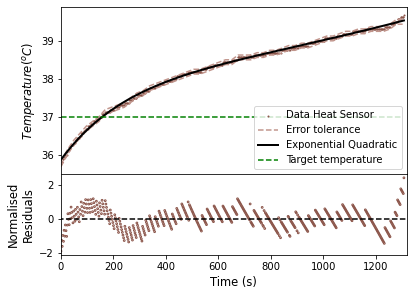
\includegraphics[width=\linewidth]{Heat sensor 23C.png}
    \caption{The plot of the roof thermocouple for a baby at 23$^{\circ}$C, with the normalised residual below. \textit{Note: Errors have been plotted as ‘bands’ outlined by the dashed lines}.}
\end{minipage}
\hfill
\begin{minipage}{.48\linewidth}
    \captionsetup{justification=centering,margin=0.5cm}
    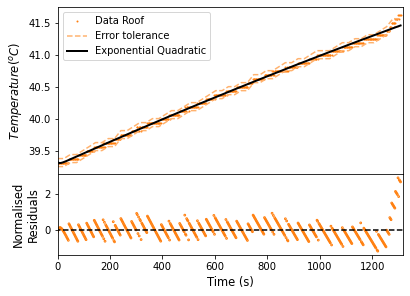
\includegraphics[width=\linewidth]{Roof 23C.png}
    \caption{The plot of the heat sensor thermocouple for a baby at 23$^{\circ}$C, with the normalised residual below. \textit{Note: Errors have been plotted as ‘bands’ outlined by the dashed lines}.}
    \label{ROOF 23C}
    \end{minipage}
\end{figure}

This caused a considerable overshooting of the temperature in all areas of the incubator. The roof data Fig. \ref{ROOF 23C} as expected, due to hot air rising, was the highest and went up to a maximum temperature of 41.625 $\pm$ 0.06$^{\circ}$C. Fig. \ref{Cross section} below shows the convection currents inside the incubator.

\begin{figure}[!h]
    \centering
    \captionsetup{justification=centering,margin=1cm}
    \includegraphics[width=0.5\textwidth]{Servo CS.png}
    \caption{A cross sectional view of the incubator, giving direction of heat flow around the system.}
    \label{Cross section}
\end{figure}

\vspace{3mm}

The heat is released around the edge of the bed inside the incubator, causing it to rise up the edges on all sides. It then collides with the hot air from the other side at the top forcing it to fall down in the middle of the incubator, where the baby is located. This caused temperatures to be higher than desired where the baby is located, up to 39 $\pm$ 0.06$^{\circ}$C. These findings confirm the nurse's initial worries about how servo mode increases the air temperature by too much. A solution to this problem would be to have more heat sensors around the incubator. This would give a more accurate representation of the temperature of the whole incubator and thus, the correct air temperature could be achieved for the baby’s specific needs.
 
\vspace{3mm}

When looking at the problem associated with the sticker, it was noted that our electrical tape, used to stick thermocouples and humidity sensors around the incubator, did in fact lose its stickiness at high temperatures and humidity values. It was concluded that this would happen for the stickers used to attach the thermocouples to the baby too. A solution could be to use a laser or infrared temperature sensor to remove the chance of the sticker falling off or irritating the baby’s skin. The limitations to this are discussed in the limitations section.

\vspace{3mm}


It was noted that the models were an over fit for the data, due to the values of $\chi^{2}_{v} < 1$ and $P(\chi^{2}_{min};v) = 1$. The most probable source of error here was overestimating the uncertainties within the data collection. Refer to the appendix for more information on the chi-square analysis (Sec. 11.2).

\section{Suggested Incubator Improvements}

One objective of this project was to suggest and prototype potential improvements to the incubators in order to enhance their functionality. The problems to be resolved were as follows: 

\begin{enumerate}

\item The nursing staff at the hospital recounted that the temperature probe that attaches to the baby during servo mode often falls off as it is only held on by a weak, gel-based sticker, designed not to damage the baby’s skin. As such, when the probe falls off, the incubator reads an inaccurate temperature for the baby, potentially activating temperature rises or falls that could be harmful. Is there a better way to secure the probe to the baby, or perhaps a better way to measure the baby’s temperature altogether? 

\item Experimental data showed that humidity impacts the heat retention of the incubator significantly (see Sec. \ref{AirModeResults}). As such, it is crucial to maintain a high humidity where possible. Our data shows humidity plummeting when the portholes are opened, which might happen during a medical procedure or for parental contact. Is there a modification that can be made to the incubator to ensure a high relative humidity is maintained while still allowing medical staff or parents to interact with the baby? 

\end{enumerate}

\vspace{3mm}

\noindent \textbf{\textit{Potential Resolutions to Problem 1}}

 \vspace{3mm}

Several methods of determining the baby’s temperature during servo mode were devised. The use of an infra-red thermal camera might be a possible method of remotely measuring the baby’s temperature without needing to be in contact with the skin. However, there is the possibility that the baby could move out of the field of view of the infra-red sensor and once again, read an inaccurate temperature. 

 \vspace{3mm}

A typical infrared sensor has a field-of-view of roughly 32 degrees (at a minimum) \cite{JG5}, therefore creating a total viewing width of 280mm, 2 s.f, at a distance of 480mm.  (see Fig. \ref{fig:IRcameraFOV}). Assuming the sensor is placed directly in the lateral centre of the incubator, this leaves roughly 10cm of space at either side of the incubator in which the baby would not be detected by the infrared sensor. This solution is therefore not perfect as there is a non-zero chance the baby could stray outside the bounds of the sensor’s visibility, hence causing inaccurate temperature readings. However the probability of this happening is unknown and would require further investigation by resident NICU medical staff.


\begin{figure}[h!]
    \centering
    \captionsetup{justification=centering,margin=0.3cm}
    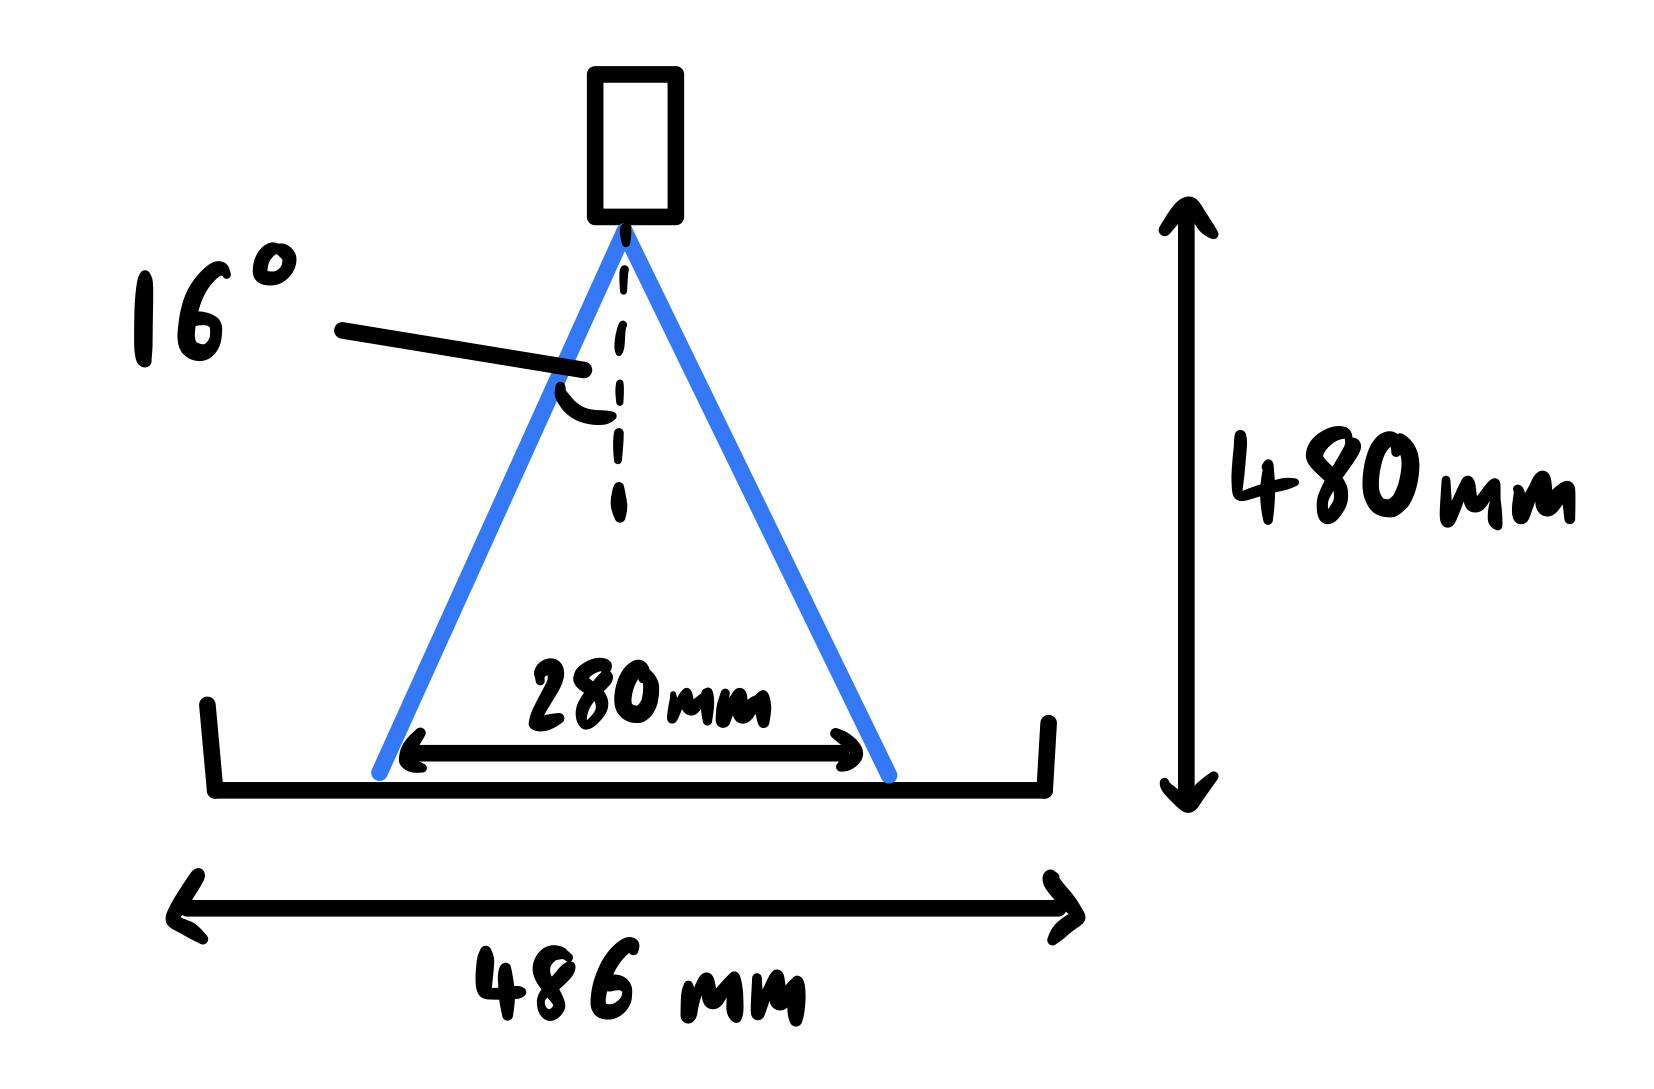
\includegraphics[width = 0.5\linewidth]{infraredcamerafov.jpeg}
    \caption{A diagram showing the front-facing field-of-view of a typical infra-red sensor when placed on the roof of the incubator that was used, with a height of 480mm and width of 486mm. This is from the frontal view (see Sec. \ref{MethodSection} for incubator diagram and referral system). }
    \label{fig:IRcameraFOV}
\end{figure}

\vspace{3mm}

It was also suggested that a UV-curing adhesive could be used to secure the probe to the baby. This method would involve a gel being applied to the baby which then hardens when exposed to UV light. Then the adhesive can be dissolved using a solvent or scrubbing with soap and water. However, this solution will most likely be unsuitable as exposure to excessive UV light is not preferable, and most glue-dissolving solvents will most likely be harmful to premature babies. Furthermore, scrubbing the skin with soap and water might cause irritation on the baby's skin that isn’t fully developed. Additionally, the medical staff at James Cook University Hospital commented that dissolving materials (e.g. stitches) do not fully dissolve in practice, and new parents will not want partially dissolved materials in or on their new-born. Further investigation is required to determine whether or not there is a suitable solvent for this purpose - one that effectively and entirely removes the adhesive while also remaining safe for the baby.

 
\vspace{9mm}
 
\newpage
\noindent \textbf{\textit{Potential Resolutions to Problem 2}}

 \vspace{3mm}

Temperature readings were taken for a low humidity of (24 ± 1) \% to (29 ± 1) \% (see section 6.2 earlier in the report for graphical results and discussion). At a higher relative humidity, the incubator retained heat a lot more effectively – a lower decrease in temperature was observed at 75\% humidity (see Sec. \ref{AirModeResults} for low-humidity data results). As such, it was attempted to devise an improvement that would decrease the drop in humidity and also retain heat better than an open porthole. 

 \vspace{3mm}

Initially, the idea of attaching rubber gloves to the portholes was proposed, such that the caregiver could insert their hands and interact with the baby without making physical contact and while creating a membrane between the inside of the incubator and the outside world. This solution would prevent a humidity drop by creating a physical barrier, as well as avoiding an increase in infection risk as rubber gloves can easily be sterilised. Certain designs of rubber gloves transmit heat poorly (for example those used for washing dishes in order to stop the user from burning their hands) and as such would provide an insulating barrier to the portholes. However, poorly fitted gloves could cause difficulties performing medical procedures (difficulty holding equipment, difficulty with mobility) - for example, the James Cook University Hospital medical staff described a procedure involving inserting lines into neonates which are approximately 1mm in diameter, hence incredible precision accuracy is required. Furthermore, fingered gloves prevent skin-to-skin contact that parents might request for bonding. As such, a solution which allows for free, un-covered fingers is required. 

 \vspace{3mm}

The next proposed idea was to cut the fingers off the gloves and create a sleeve that fitted tightly around the wrists. It was suggested that the sleeve from a woollen jumper was used as it would be effective at maintaining heat, however fibrous material introduces a significant infection risk and is therefore inappropriate. It was raised that woollen clothes insulate by trapping a layer of air that acts as an insulator, hence bubble wrap (or a material of a similar nature, likely rubber due to its ability to create a seal) would be appropriate for these finger-less sleeves. This allows for an insulating layer of air while keeping the ability of being sterilised and also allowing for skin-to-skin contact with the baby. This bubble wrap design was tested on our own model incubator and caused significant improvements in heat and humidity retention. See Sec. \ref{ModelForImprovements} for more details.  

\section{Creating a model to test for improvements} \label{ModelForImprovements}

\subsection{Introduction} \label{ModelSecIntro}
In this section will be a discussion of a possible improvement that can be made the incubator in order to reduce heat and humidity loss. 

\vspace{3mm}

A model for a cooling system with no heat source is given by Newton’s law of cooling, formulated in 1701 \cite{JR1} \cite{JR2},
\begin{equation} \label{NewtonDerivative}
    \frac{dT}{dt} = -k(T-Ta),
\end{equation}

Which states that the cooling rate is proportional to the difference in temperature between the system, $T$, and ambient, $Ta$, by a transfer coefficient $k$. There is a $T-Ta$ dependence as the system and surroundings are considered to have a boundary of still (i.e. not moving) fluid between them the system must heat, which is then carried away by convection. Therefore, the properties of both the system and surroundings affect the cooling, hence the dependence of $T-Ta$.
Solving this for a system warmer than ambient,

\begin{equation} \label{NewtonianCooling}
    T(t) = Ce^{-kt} +T_a,
\end{equation}

where $C$ is a constant associated with Newtonian cooling, and $k$ is a decay constant. To account for a system not cooling to the same temperature as the ambient (to equilibrium) an extra constant is added,

\begin{equation} \label{GeneralNewtonianCooling}
    T(t) = Ce^{-kt} +T_a + A.
\end{equation}
In this form of an exponential, $C$ determines after what time the cooling plateaus, $k$ determines the steepness of the transition from the cooling to the plateau, and A determines final temperature.

\vspace{3mm}
To test the efficacy of any improvements made to the incubator, the temperature curve of the previously mentioned model incubator was fitted to General Newtonian cooling  Eq. \ref{GeneralNewtonianCooling}, and coefficients compared as well as a comparison of ranges and general trends. The humidity of the system is also an important factor of the thermodynamic behaviour of the system. However, the data was fitted to an arbitrary model to compare the parameters for discussion, as well as ranges and trends.
The improvement thought to have the largest effect would be a skin-tight gasket on the incubator portholes. This would cause a seal between the user’s arm reducing humidity loss and eliminating convection flow out of the portholes, while still allowing skin to skin contact with the user and baby and allow for better dexterity than a gloved design. 


\subsection{Additional Methodology}



The standard trial methodology is followed, the same control and 2 open doors experiments were carried out on the model.
\vspace{3mm}

\begin{figure}[!h]
    \centering{}
    \captionsetup{justification=centering,margin=0.3cm}
    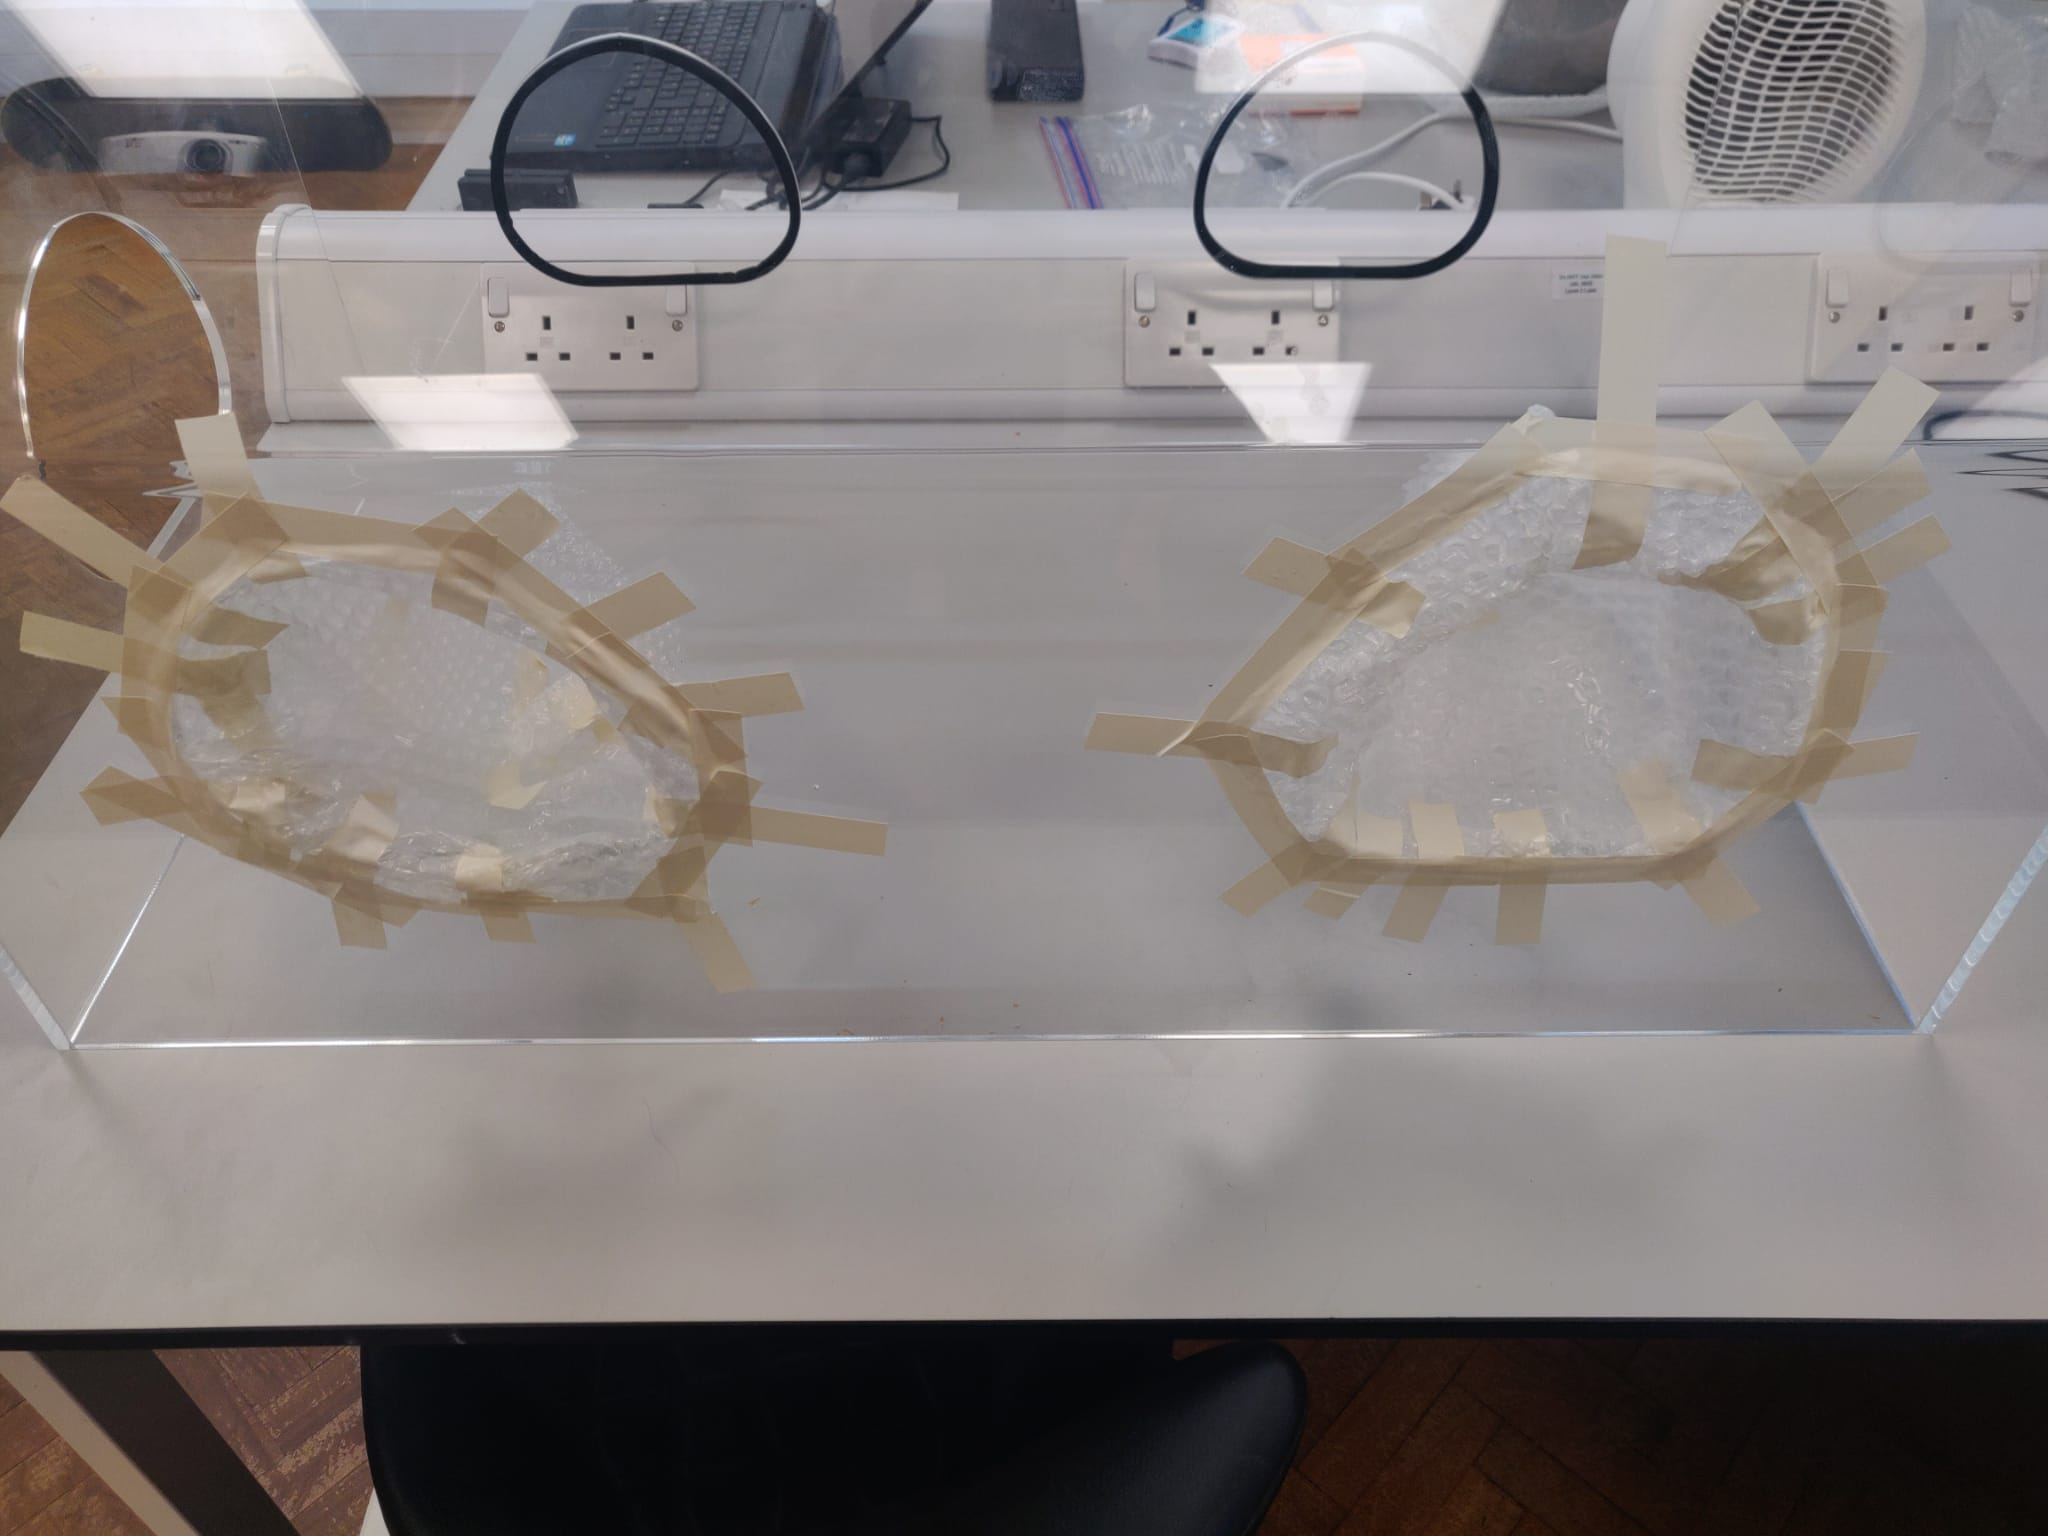
\includegraphics[width=0.5\textwidth]{PicOfSleeves.jpeg}
    \caption{Photo of the portholes with affixed sleeves}
    \label{fig:PicOfSleeves}
\end{figure}


The trials conducted with the 2 doors open, both with and without sleeves are considered the experimental trials.
The proposed gaskets were realised as sleeves made of bubble wrap which were attached and sealed with electrical tape to the same 2 doors on the model used for the non-sleeved trial, Fig. \ref{fig:PicOfSleeves}. Bubble wrap and electrical tape were used due to their insulating properties, the bubble wrap containing air pockets and the tape being rubberised and made for insulation.
\vspace{3mm}

The standard experimental protocol was then conducted on this experimental setup. 
The gaskets are used to seal around a person’s arms, as in a hospital setting the portholes are used for access into the incubator to care for the baby. Therefore, the portholes had arms through them for both experimental trials to control for their use both in real applications and between experiments, as the gaskets will be most effective when sealed around an arm. 


\subsection{Results}

\begin{figure}[h!]
\centering
\begin{subfigure}{0.48\textwidth}
\centering{}
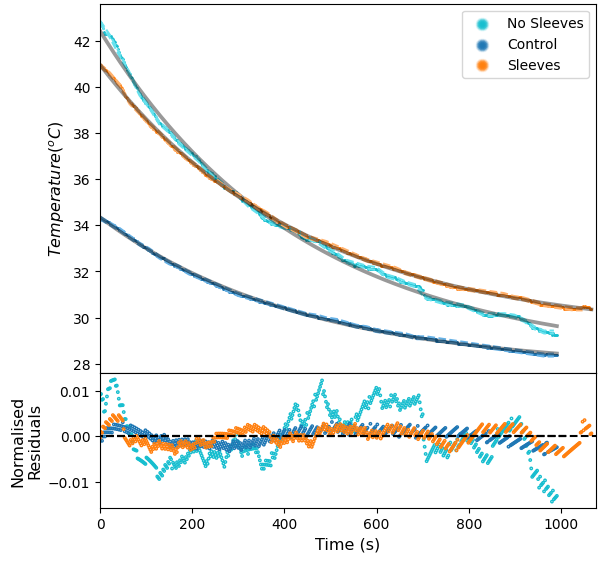
\includegraphics[scale = 0.3]{LeftTmp.png} 
\caption{Left Porthole}
\label{fig:ModTmpPlotLeft}
\end{subfigure}
\begin{subfigure}{0.48\textwidth}
\centering{}
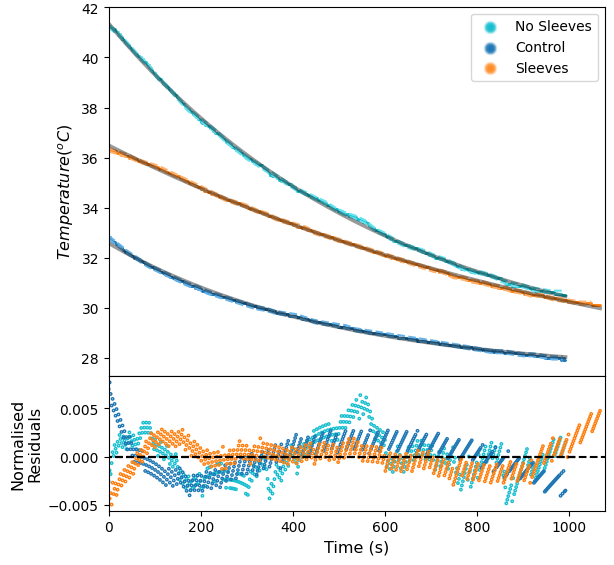
\includegraphics[scale = 0.3]{RightTmp.png}
\caption{Right Porthole}
\label{fig:ModTmpPlotRight}
\end{subfigure}
\captionsetup{justification=centering,margin=0.3cm}
\caption{Temperature ($^{\circ}$C) by time (s) of temperature probes at portholes with  dashed error range, with the Eq. \ref{GeneralNewtonianCooling} model as a black line, with residuals.}
\label{fig:ModTmpPlot}
\end{figure}

\begin{figure}[h]
    \centering
    \captionsetup{justification=centering,margin=0.3cm}
    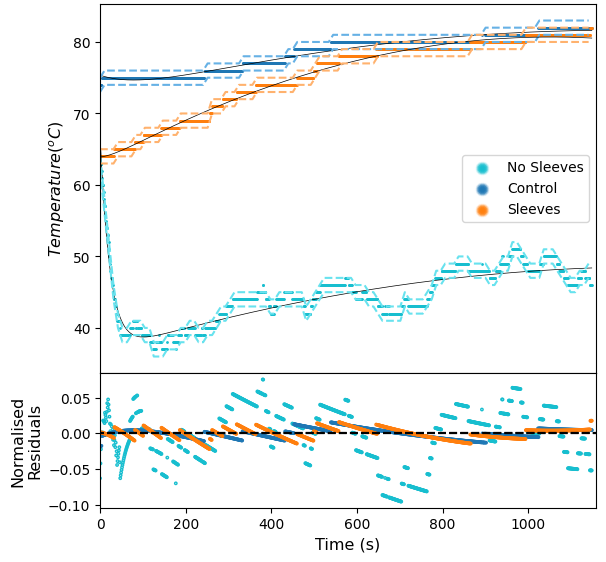
\includegraphics[scale = 0.3]{Hum.png}
    \caption{Humidity ($\%$) by time (s) of the model incubator for each trail with a dashed error range, with the Exponential Cubic model as a black line, with residuals.}
    \label{fig:ModHumPlot}
\end{figure}


\begin{figure}[h]
    \centering{}
    \captionsetup{justification=centering,margin=0.3cm}
    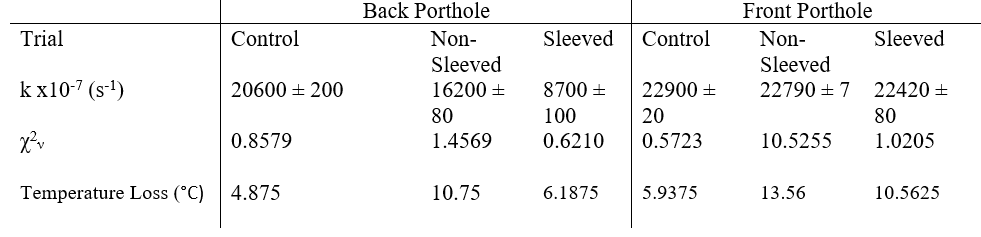
\includegraphics[scale = 0.5]{ModTmpTable.png}
    \caption{A table of $k$ with error ($\times10^{-7}s^{-1}$) for all trials at each porthole, with reduced chi squared, $\chi^2_\nu$, and loss of temperature with error $\pm0.0625$}
    \label{fig:ModTmpTable}
\end{figure}

\begin{figure}[!h]
    \centering{}
    \captionsetup{justification=centering,margin=0.3cm}
    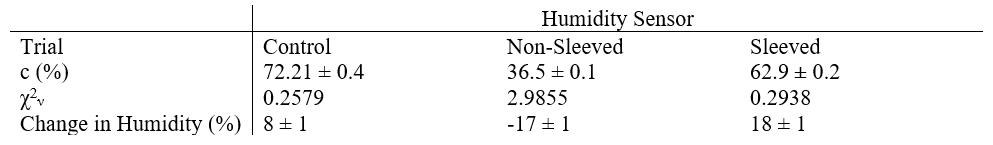
\includegraphics[width = 0.9\linewidth]{ModHumTable.png}
    \caption{Parameter $c$ ($\%$) of all trials modelled by exponential cubic Exponential Cubic, and change in humidity, with reduced chi squared, $\chi^2_\nu$, and change in humidity }
    \label{fig:ModHumTable}
\end{figure}



Possibly due to changes in resistance due to heat and humidity, the trails in this section ran for 16 minutes rather than 20 minutes. The ambient temperature was recorded for the model trials to be $T_a = 21 \pm 1^{\circ}$C using a temperature installed on the room wall. The data was then fitted to the generalised Newtonian cooling Model Eq. \ref{GeneralNewtonianCooling}, the results are tabulated in Fig. \ref{fig:ModTmpPlot} and graphed with the model fitted shown as a thin black like in Fig. \ref{fig:ModTmpPlot}. 
For the humidity results, the ambient humidity was measured to be $47 \pm 1\%$. The data was then fit best to an exponential decay model with a quadratic added as in Exponential Cubic, the parameters are shown in Fig. \ref{fig:ModHumPlot} and the data and model are plotted in Fig. \ref{fig:ModHumPlot}.

\newpage
\subsection{Discussion}

$C$ and $A$ of  Eq. \ref{GeneralNewtonianCooling} only act to translate the plot, so they are not significant for consideration, so only k will be discussed as it is the decay constant in  Eq. \ref{GeneralNewtonianCooling}.  Also, as this experiment was to test the efficacy of the reduction in temperature and humidity loss through the portholes via affixing a gasket, data from the portholes will be the focus of discussion, as this experiment is testing the reduction in temperature and humidity lost from the portholes with gaskets attached.

\vspace{3mm}
As previously stated in Sec. \ref{AirModeBoostSection}, the incubator is high effective at maintaining both humidity and temperature. But as can be seen from Fig. \ref{fig:ModTmpPlot} the model lost heat both in the control and with 2 doors open. The model however did manage to maintain humidity in the control, as the humidity was physically unable to leave. Reviewing the data, the model would not be a good stand in for an actual incubator. This will be due to the lack of an active heater and humidifier running during the time of use, as well as well sealed insulation around the portholes. As should the model is only used to review the efficacy of the experimental alterations made in this report, against itself as to suggest improvements to be made to the real incubator.

\vspace{3mm}
For all trails on both incubators, including the control, $k$ was almost always in a range of 0.0015s$^{-1}$ to 0.0023s$^{-1}$ range. The only significant reduction is for the back porthole when sleeved, $k$ dropping to $0.00087 \pm 1\times10^{-5}$ s$^{-1}$. This causes a later plateau point for the cooling curve, implying greater heat retention.

\vspace{3mm}
Fig. \ref{fig:ModTmpTable} has the losses in temperature for the trials at each porthole. For the non-sleeved trial there were losses of over $10.7^{\circ}$C but the sleeved trials largest drop was only 10.56 $\pm$ 0.06$^{\circ}$C, meaning the highest change with sleeves is less than the lowest change without sleeves.  

\vspace{3mm}
As can be easily seen from Fig. \ref{fig:ModHumPlot} the humidity for the control and sleeved trail, the humidity increased, as opposed to only maintaining a constant value. Whereas in the non-sleeved trials the humidity dropped a large amount at the start. 
Parameter c in Exponential Cubic is the determining parameter in final humidity, as it is a linear term that translates the curve in the y-axis (humidity). The value of c for the control is double that of the non-sleeved trials, meaning the final humidity was significantly less for the non-sleeved trials, as can be seen in Fig. \ref{fig:ModHumPlot}. The value of c in the sleeved trials is only $9.311\%$ less than the control (this is an absolute difference, not relative), so it is a significant improvement to no sleeves.

\subsection{Conclusion}
In conclusion, the data suggests attaching sleeves to the portholes on the incubator has the effect of reducing temperature loss by between $3^{\circ}$C - $4^{\circ}$C at the portholes. Adding sleeves also significantly reduces the loss of humidity, which, as seen before in Air Boost, is a major factor in the heat retention of the incubator. As any loss in temperature can be dangerous in this context, a full examination of modifying incubators to have some form as gasket is suggested by out data.



\section{Overall Conclusion}
\vspace{3mm}

When studying the effects of Servo mode, it was clear that the incubator effectively increased the temperature inside for a baby whose skin temperature was below the set value and reduced the incubator's overall temperature for an overheating baby. The incubator found it easier to increase than decrease its temperature over the period of time experimented. The speed of the incubators response is proportional to the difference between the set temperature and the actual temperature of the baby. 

\vspace{3mm}

When using 'air mode', the temperature of the baby model was not able to reach the target temperature when 2 or 4 portholes were opened, and remained at critical temperatures posing a high risk of hypothermia to the baby. Therefore, to mitigate these effects, it is suggested while using a configuration of open portholes, to set a target temperature higher than the desired temperature to allow for heat loss through these porthole doors. Furthermore, setting a humidity higher than the desired humidity will also reduce the effects of humidity loss. However, when all porthole doors were closed, 'air mode' was effective at heating the model of the baby to the target temperature and maintaining heat in the incubator.

\vspace{3mm}

Over the course of the 20 minute period, the temperature of the baby remained constant at 35$^{\circ}$C, approximately 2 $^{\circ}$C lower than the set temperature of the air. This is true for both ‘Air boost’ and ‘Air mode’. The most significant source of the heat loss arises at the end of the incubator. ‘air boost’ does appear to decrease humidity at a much faster rate than ‘air mode’. This is potentially due to the power of the air coming from the heater being stronger when using ‘air boost’, causing more humid air to be lost through the portholes. In turn this may lead to issues over long periods, as humid air has a higher thermal mass and thus can hold more energy to be transferred to the neonate. Therefore, a system after the humidity has significantly declined may be much less thermally stable suggesting that for long term thermal stability, it may be more useful to ‘air mode’ than ‘air boost’ unless there is a significant decline in temperature.

\vspace{3mm}

Over the 20-minute measuring period, with 4 portholes open, 'air boost' caused the temperature under the baby to fluctuate with an amplitude of roughly 0.5$^{\circ}$C, whereas 'air mode' by itself exhibited a steady maintenance of temperature within $\pm$ 0.5$^{\circ}$C. In 'air mode,' the temperature at the end porthole dropped more drastically than the others, approaching 32$^{\circ}$C and suggested a further drop was imminent. However, 'air boost' reached a minimum end porthole temperature of roughly 33.5$^{\circ}$C at roughly 10 minutes before then steadily rising again. This result is promising as it suggests air boost prevents an air temperature decrease into critically cold levels. Humidity dropped to a lower level with air boost enabled compared to regular air mode. Humidity is essential for the retention of heat, and hence a greater decrease is not preferable, however air boost results conveyed that temperature was still maintained well despite this due to the larger influx of warm air into the incubator.

\vspace{3mm}

At lower humidity levels, the heat loss through the porthole doors were slightly reduced, resulting in a higher temperature at the top of the incubator. However, both results with high or low humidity levels had negligible effect on increasing the temperature of the baby model to the target temperature when using ‘air mode’, therefore, humidity was not a significant factor to the heat loss in our experiment.


\printbibliography

\newpage

\section{Appendix}

\subsection{Arduino Circuit Diagrams}


A common 5V live and ground channel were created on a breadboard by  plugging in the 5V live and ground source from the Arduino (a small computer) into a breadboard (a board for connecting wires). The thermocouples (6 or 7) were plugged into the common live and ground channels, each had an error of $\pm0.0625^{\circ}$C. The data wires of all the thermocouples were plugged into individual channels in the breadboard, which are connected together in series. Then, a 4.7k$\Omega$ resistor was connected from common live to the bottom of the series of data wires, and the top of the series was connected to the Arduino D2 digital in channel. This is shown in Fig. \ref{fig:CircuitDiagramsThermo}.

\vspace{3mm}

As well as this, a different Arduino was used for a live and ground channel are created as above, however 2 humidity sensors, with error of $\pm1\%$ humidity, were connected, and then their data wires were connected directly to the D2 and D3 digital in channels on this Arduino. This is shown in fig. \ref{fig:CircuitDiagramsHum}.

\begin{figure}[H]

\begin{subfigure}{0.5\textwidth}
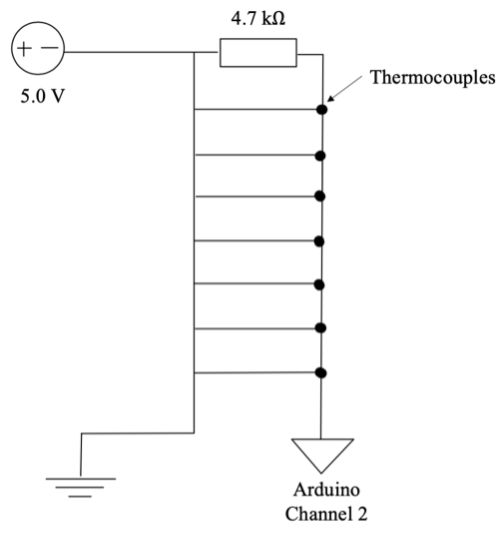
\includegraphics[scale = 1]{Thermocouple circuit.png} 
\caption{The thermocouple circuit diagram.}
\label{fig:CircuitDiagramsThermo}
\end{subfigure}
\begin{subfigure}{0.5\textwidth}
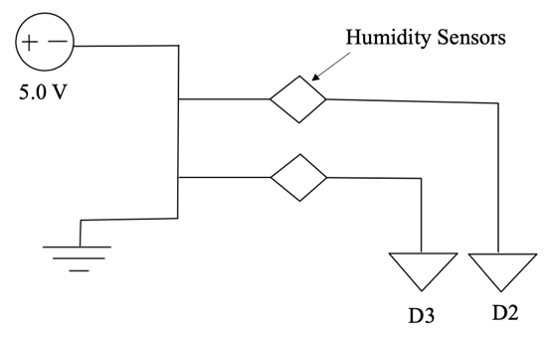
\includegraphics[scale = 1]{Humidity Circuit.png}
\caption{The humidity circuit diagram.}
\label{fig:CircuitDiagramsHum}
\end{subfigure}

\caption{Circuit Diagrams for the data collecting Arduinos.}
\label{fig:CircuitDiagrams}
\end{figure}



The Arduino  measuring temperature ran a program that would record the temperature of a thermocouple, print  the serial and repeat until it had printed all the readings from all the probes, and repeated this until shut off.
The Arduino measuring humidity ran a program that would get the humidity reading from the probe attached to the D2 channel and print it to the serial, then did the same for the D3 channel, and repeat until shut off. 


\vspace{3mm}

Then as instructed in the experimental planning , as given in Sec. \ref{MethodSection}, the python data logging programs were then set to run for the time allotted to that experiment (20 min) via taking a corresponding number of readings for both the thermocouples and humidity sensors by reading the serial of the Arduinos (4350  readings for the Arduino measuring temperature, 1200 readings for the Arduino measuring humidity).

\vspace{3mm}

This data was then sent from the Arduino to a computer running the data logger into a pandas data frame and saved as a .csv file, along with a UNIX time stamp of the local time and time elapsed, so it was known when each datum was collected given the first measurement calculated in the logging program. 

\subsection{Chi-Square Tests and Error analysis}

Chi squared tests are used to fit a given set of data to a specified model function \cite{LS2}. The chi-squared value, $\chi^{2}$, then shows the goodness of fit of these parameters and is given by the equation:

\begin{equation}\label{ChiEqn}
\chi^{2} = \sum_{i}\frac{(y_{i}-y(x_{i}))^{2}}{\alpha_{i}^{2}},
\end{equation}

where  $y_{i}$ is the measured y-values from the data set, $y(x_{i})$ is the y-values calculated by the model function, and $\alpha_{i}$ is the error in the data point, $y_{i}$. The chi-squared value is equivalent to the sum of the square of normalised residuals. To show a model function fits the data set is suitable, the reduced chi-squared value, $\chi_{\nu}^{2}$, should be approximately equal to 1 (Please refer to section ... for model functions used). The reduced chi-squared value is given by:

\begin{equation}\label{ReducedChiEqn}
\chi_{\nu}^{2} = \frac{\chi^{2}}{\nu},
\end{equation}

where $\nu$ is the degrees of freedom. A reduced chi-squared value significantly greater than 1 shows the model function is not suitable to fit the data set and should be rejected. A reduced chi-squared value of less than 1 shows the discrepancy between the data set and the model function is smaller than expected by the error stated. This suggests the error, $\alpha_{i}$, may be inaccurate and is smaller than previously stated.

\vspace{3mm}

For the relationship between the temperature with increasing time period, the error, $\alpha_{i}$ ($\pm$ 0.0625 $^{\circ}$C), in Eq. \ref{ChiEqn} is taken as the uncertainty of the thermocouple given by the manufacturer. This relationship is fitted to various model functions using chi-squared tests. The model functions selected are ones that give the minimum chi-squared value, therefore, the most suitable fit for the data set. The error, $\alpha_{i}$, also corresponds to the vertical error bars in figures with a plot of the temperature.

\vspace{3mm}

The majority of temperature data sets that was measured using the incubator at the James Cook University Hospital was fitted the Exponential Cubic model function with a few exceptions (Please refer to Sec. \ref{MethodSection} for model functions). The data collected from our model incubator in the physics department was fitted to Eq. \ref{GeneralNewtonianCooling} which is given in Sec. \ref{ModelSecIntro}.

\vspace{3mm}

For the relationship between the humidity with evolving time period, the error, $\alpha_{i}$ ($\pm$1\%), in Eq. \ref{ChiEqn} is taken as the uncertainty in the humidity sensor quoted by the manufacturer. All humidity data sets for 'air mode', 'air boost' and 'servo mode' were fitted to an exponential linear model function given in Fig. \ref{ModelFunctTable}

\vspace{3mm}

There was an error associated with each parameter when they were averaged in the Servo mode section \cite{LS2}. Each individual parameters error, $\alpha_{parameter}$, had to be propagated using the formula below,

\begin{equation}\label{ErrorEqn}
\alpha_{parameter} = \sqrt{\alpha_{a}^{2}+\alpha_{b}^{2}+\alpha_{c}^{2}+\alpha_{d}^{2}+\alpha_{e}^{2}+\alpha_{f}^{2}},
\end{equation}

where $\alpha_{a}$, $\alpha_{b}$, $\alpha_{c}$, $\alpha_{d}$, $\alpha_{e}$ and $\alpha_{f}$ are all the individual uncertainties of the parameter for each of the 6 thermocouples.

\vspace{3mm}

For some of the residuals which displayed multiple diagonal straight lines, this is due to the digital nature of the thermocouples and the humidity sensors. Therefore, as some data sets had a narrow range of temperatures or humidity, the precision of these devices caused these residual trends when it was approximated to a continuous model function.  However, other trends in residuals were not significant, confirming the model function is a suitable fit to the given data set.

\vspace{3mm}

Furthermore, for the data sets that have a reduced chi-squared value that is larger than 1, this is likely due to the fluctuation caused by the incubator settings changing through different temperatures. However, the model function was chosen to approximate the best trend the data sets displayed despite these fluctuations. 

\subsection{Methodology}

\begin{figure}[h]
\centering
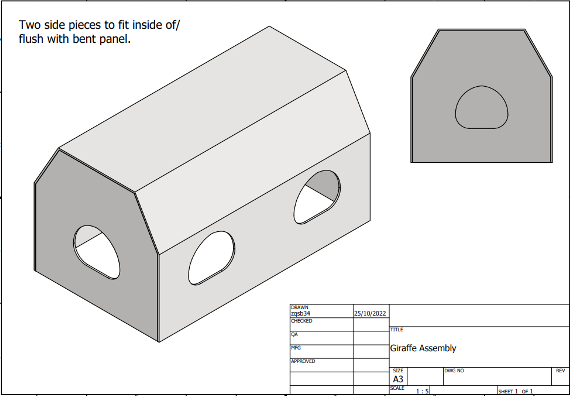
\includegraphics[width=.4\textwidth]{Model 1.png}\quad
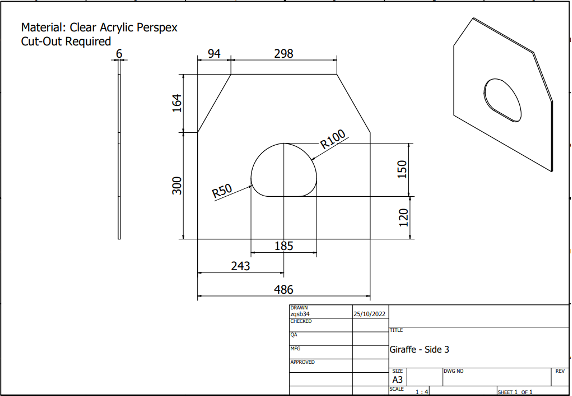
\includegraphics[width=.4\textwidth]{Model 2.png}

\medskip

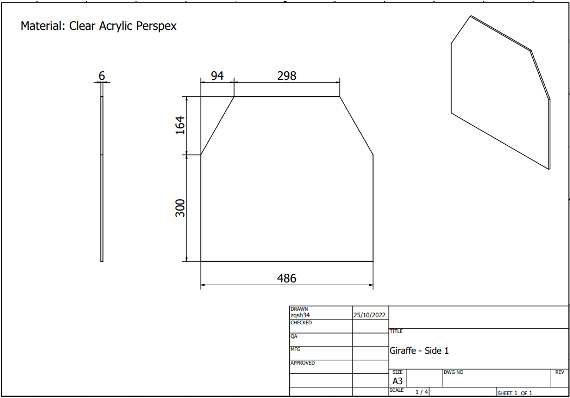
\includegraphics[width=.4\textwidth]{Model 3.png}\quad
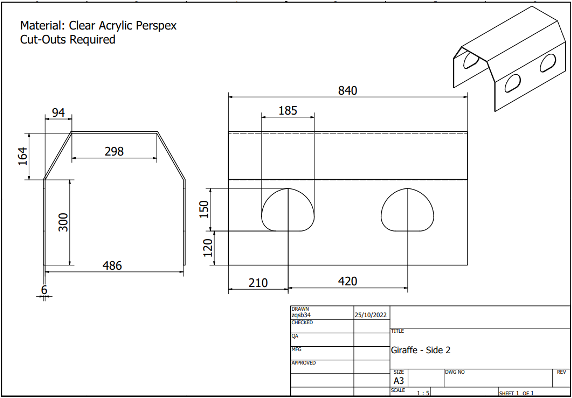
\includegraphics[width=.4\textwidth]{Model 4.png}
\captionsetup{justification=centering,margin=0.3cm}
\caption{Diagram of the acrylic model of the GI Giraffe Incubator Produced by Durham University Physics Workshop Team} 
\label{Acrylic model}
\end{figure}

\subsection{Board meeting minutes}



\newpage
\thispagestyle{empty}
\mbox{}
\newpage
\newpage
\thispagestyle{empty}
\mbox{}
\newpage
\newpage
\thispagestyle{empty}
\mbox{}
\newpage
\newpage
\thispagestyle{empty}
\mbox{}
\newpage
\newpage
\thispagestyle{empty}
\mbox{}
\newpage
\newpage
\thispagestyle{empty}
\mbox{}
\newpage
\newpage
\thispagestyle{empty}
\mbox{}
\newpage
\newpage
\thispagestyle{empty}
\mbox{}
\newpage
\thispagestyle{empty}
\mbox{}
\newpage
\newpage



\section{Scientific Summary for a General Audience}
Premature children have difficulty maintaining temperature due to their lack of heat producing functions, they therefore are placed in heat producing incubators. However, these incubators must often be opened (using porthole doors) to allow investigation or medical procedures on the baby to occur. This provides a significant means of heat loss, which if too severe, can cause harm and illness to the new-born. It was found  that servo mode was incredibly effective at maintaining internal temperature, to the extent of potentially heating above the desired temperature. ‘Air boost’ and ‘air mode’ were both effective at maintaining temperature, although the model baby in both cases remained 1.5-2.0 °C colder than the target temperature. The report suggests within 20 minutes of opening any combination of portholes, the neonate does not fall significantly in temperature and ‘air boost’ after the portholes are closed effectively recoups temperature, however further works should be done to ascertain the temperature decline for longer periods of time. 



\end{document}
